\documentclass{cernrep}
%% Language and font encodings
\usepackage[english]{babel}
\usepackage[utf8x]{inputenc}
\usepackage[T1]{fontenc}

%% Sets page size and margins
\usepackage[a4paper,top=3cm,bottom=2cm,left=3cm,right=3cm,marginparwidth=1.75cm]{geometry}

%% Useful packages
\usepackage{amsmath}
\usepackage{graphicx}
\usepackage[colorinlistoftodos]{todonotes}
\usepackage[colorlinks=true, allcolors=blue]{hyperref}
\pagestyle{plain}
\newcommand{\Zp}{\ensuremath{Z^{\prime}}}
\newcommand{\ZpSSM}{\ensuremath{Z^{\prime}_{\mathrm{SSM}}}}
\newcommand{\Z}{\ensuremath{Z}}
\newcommand{\ttbar}{\ensuremath{t\bar{t}}}
\newcommand{\ptSub}[1]{\ensuremath{p_{\text{T} #1}}}
\newcommand{\ptSup}[1]{\ensuremath{p_{\text{T}}^{#1}}}
\newcommand{\pt}{\ensuremath{p_{\text{T}}}}
\newcommand{\ptEl}{\ensuremath{p_{\text{T}}^{e}}}
\newcommand{\ptMu}{\ensuremath{p_{\text{T}}^{\mu{}}}}
\newcommand{\ptZp}{\ensuremath{p_{\text{T}}^{\ensuremath{Z^{\prime}}}}}
\newcommand{\mZp}{\ensuremath{M_{\ensuremath{Z^{\prime}}}}}
\newcommand{\mll}{\ensuremath{M_{\ensuremath{ll}}}}

\def\ifb{\mbox{fb$^{-1}$}}%  Inverse femtobarns.
\def\afb{\mbox{ab$^{-1}$}}%  Inverse femtobarns.

\def\TeV{\ifmmode {\mathrm{\ Te\kern -0.1em V}}\else
                   \textrm{Te\kern -0.1em V}\fi}%
\def\GeV{\ifmmode {\mathrm{\ Ge\kern -0.1em V}}\else
                   \textrm{Ge\kern -0.1em V}\fi}%
\def\MeV{\ifmmode {\mathrm{\ Me\kern -0.1em V}}\else
                   \textrm{Me\kern -0.1em V}\fi}%
\def\keV{\ifmmode {\mathrm{\ ke\kern -0.1em V}}\else
                   \textrm{ke\kern -0.1em V}\fi}%
\def\eV{\ifmmode  {\mathrm{\ e\kern -0.1em V}}\else
                   \textrm{e\kern -0.1em V}\fi}%


\begin{document}
\title{FCC Physics: Heavy resonances $\Zp$, RS graviton at $\sqrt{s} = 100 \TeV$}
\author{Clement Helsens${}^1$,\,
David Jamin${}^1$,\,
Michele Selvaggi${}^1$}
\institute{${}^1$ CERN, Geneva, Switzerland}

%di-jet
%https://arxiv.org/pdf/1703.09127.pdf
%ATLAS INT NOTE ttbar res 
%https://cds.cern.ch/record/1640960/files/ATL-COM-PHYS-2014-003.pdf

\begin{abstract}
This paper explores the physics reach of the proton-proton Future Circular Collider (FCC-hh)
for searches of new particles decaying to two high energetic leptons, tops or W/Z boson. We discuss the expected exclusion limits and discovery potential for benchmark models 
predicting new massive particles that result in resonant structures in
the invariant mass spectrum. The study is based on the Madgraph5 and Pythia8 Monte Carlo generators using large event statistics for the FCC running conditions. 
Its unprecedented  
This document presents a detailed study on the discovery potential of heavy gauge resonance $\Zp$ and center of mass energy $\sqrt[]{s} =100$~TeV makes it the ultimate machine for such new particles, and are also extremely relevant to discuss the main limitations of the detector to tag high energetic top-quarks or W/Z bosons.
\end{abstract}
\keywords{CERN report; FCC.}
\maketitle
\tableofcontents

\section{Introduction}
The design of a 100 TeV proton-proton collider leads to many challenges for detector design. Detailed optimizations of the detector is needed in order to achieve the required physics goals. The capabilities of such a detector should include the capabilities of measuring multi-TeV leptons, top-quarks and bosons.

\section{FCC work flow}
\subsection{Monte-Carlo production}
All the signal Monte-Carlo events have been produced directly with Pythia 

\subsection{Detector parameterizations}
The FCC study group is using the Delphes software package to emulate the response a detector. 
For the FCC one the baseline parameters are:
We also consider two variations around it as well as the CMS configuration.


\subsection{Multi-Variate based selection}
When relevant, in some analyses, a Multi-Variate selection will be performed using the TMVA toolkit.

- design 2 taggers to perform Whad (p8\_pp\_RSGraviton\_20TeV\_ww VS ) and thad (p8\_pp\_Zprime\_20TeV\_ttbar) separation with QCD (p8\_pp\_jj\_lo)
- made pythia independent samples from analysis, QCD has been produced to avoid useless events and to perform that the filtering has been chosen to ensure to have similar signal leading jet $\pT$ (pTHatMin = 2500, bias2Selection = on, bias2SelectionPow = 6.)
- the statistics obtained for Whad, thad and QCD are respectively 1M, 1M and 920k events with 2 jets, each jet will be an entry for the BDT training,
%- the BDT parameters for training are : !H:!V:NTrees=600:MaxDepth=4:BoostType=AdaBoost:AdaBoostBeta=0.15:SeparationType=GiniIndex:nCuts=100:PruneMethod=NoPruning
- a training selection is applied to remove uselees events with isolated leptons and jets for which jet $\tau$ ratio variables failed (i.e has a negative value)
- the training statistics obtained for Whad, thad and QCD are respectively 1117500, 1432192 and 1578098 jets, half of the stat is used for training and the other half for testing
- the variables are defined to be the same as the ones used to perform cut-based associated analysis ($\Zp \rightarrow \ttbar$ in section~\ref{subsec:Zptt} and $G \rightarrow WW$ in section~\ref{subsec:RSGww} ) and the idea is to fully exploit these informations thanks to the BDT, variable list and ranking in table~\ref{tab:TMVA_summary}

- the BDT performances 
- removing fully correlated variables have tried and doesn't change anything to performances shown
- the BDT response has been shown (\ref{fig:BDT_signal_shape_comparison}) for different signal masses generation to see how much analysis can be mass dependent. From the cuts defined in the analysis level at 0.15, the BDT shape reponse difference is not changing so much the proportion of signal kept and it removes 90\% and 95\% of QCD for thad and Whad taggers respectively

\begin{tabular}{|c|c|c|}
\hline
\hline			
 & Whad/QCD & thad/QCD \\
\hline                        
\hline                        
Sample signal     & p8\_pp\_RSGraviton\_20TeV\_ww & p8\_pp\_Zprime\_20TeV\_ttbar \\
Sample background & \multicolumn{2}{c|}{p8\_pp\_jj\_lo} \\
\hline      
Gen stat. signal (events)     & 1M & 1M \\
Gen stat. background (events) & \multicolumn{2}{c|}{920k} \\
\hline
train sel. &  \multicolumn{2}{c|}{no isolated leptons} \\
           &  \multicolumn{2}{c|}{$\tau_{21}>0$} \\
           &  \multicolumn{2}{c|}{$\tau_{31}>0$} \\
           &  \multicolumn{2}{c|}{$\tau_{32}>0$} \\
\hline
Train stat. signal (jets)     & 1117500 & 1432192  \\
Train stat. background (jets) & \multicolumn{2}{c|}{1578098} \\
\hline
BDT params  &  \multicolumn{2}{c|}{NTrees=600, MaxDepth=4, AdaBoost, AdaBoostBeta=0.15,} \\
            &  \multicolumn{2}{c|}{SeparationType=GiniIndex, nCuts=100, PruneMethod=NoPruning} \\
\hline
ranked variables & Jet\_trk02\_tau3 (0.12)        & Jet\_trk02\_tau1 (0.21) \\
                 & Jet\_trk02\_SD\_Corr\_m (0.11) & Jet\_trk02\_SD\_Corr\_m (0.17) \\
                 & Jet\_trk02\_tau31 (0.10)       & Jet\_trk02\_tau31 (0.11) \\
                 & Jet\_Flow55 (0.09)             & Jet\_trk02\_tau2 (0.10) \\
                 & Jet\_Flow45 (0.09)             & Jet\_trk02\_tau3 (0.09) \\
                 & Jet\_Flow15 (0.08)             & Jet\_trk08\_SD\_Corr\_m (0.09) \\
                 & Jet\_Flow25 (0.07)             & Jet\_trk04\_SD\_Corr\_m (0.09) \\
                 & Jet\_Flow35 (0.06)             & Jet\_trk02\_tau32 (0.08) \\
                 & Jet\_trk02\_tau21 (0.06)       & Jet\_trk02\_tau21 (0.06) \\
                 & Jet\_trk08\_SD\_Corr\_m (0.06) &  \\
                 & Jet\_trk04\_SD\_Corr\_m (0.06) &  \\
                 & Jet\_trk02\_tau1 (0.05)        &  \\
                 & Jet\_trk02\_tau2 (0.04)        &  \\
                 & Jet\_trk02\_tau32 (0.02)       &  \\
\hline
\hline
\caption{Summary of BDT informations used to train Whad/thad VS QCD.}
\label{tab:TMVA_summary}
\end{tabular}

\begin{figure}[!htb]\centering
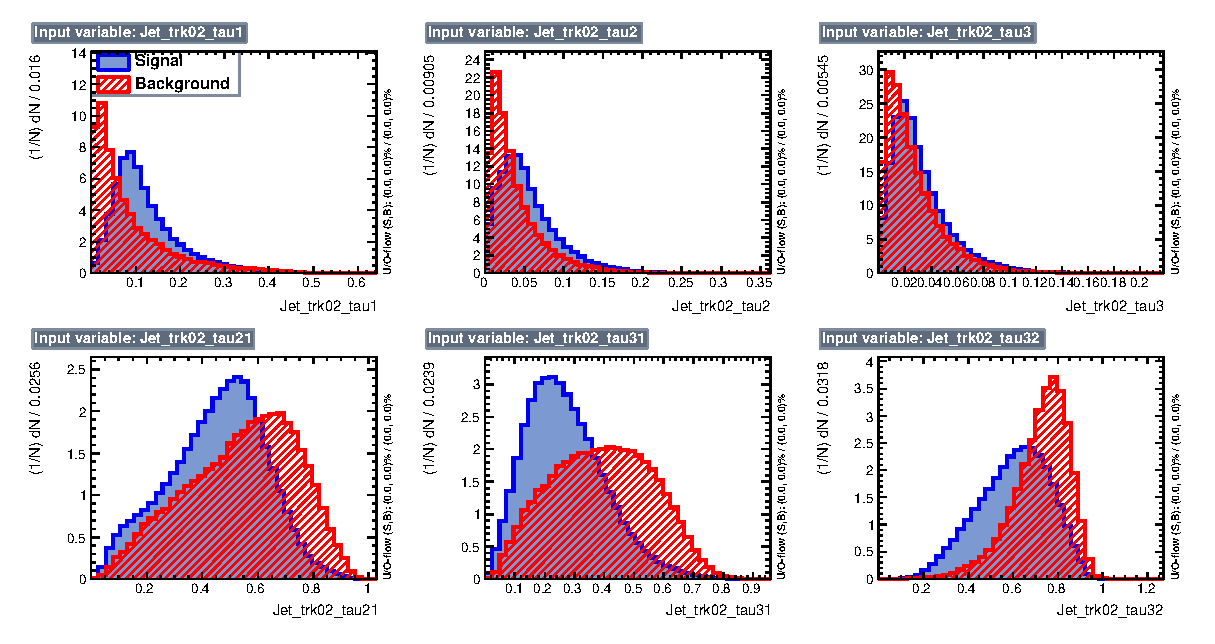
\includegraphics[width=0.495\textwidth]{Fig/TMVA/thad_vs_QCD/variables_id_c1.eps}
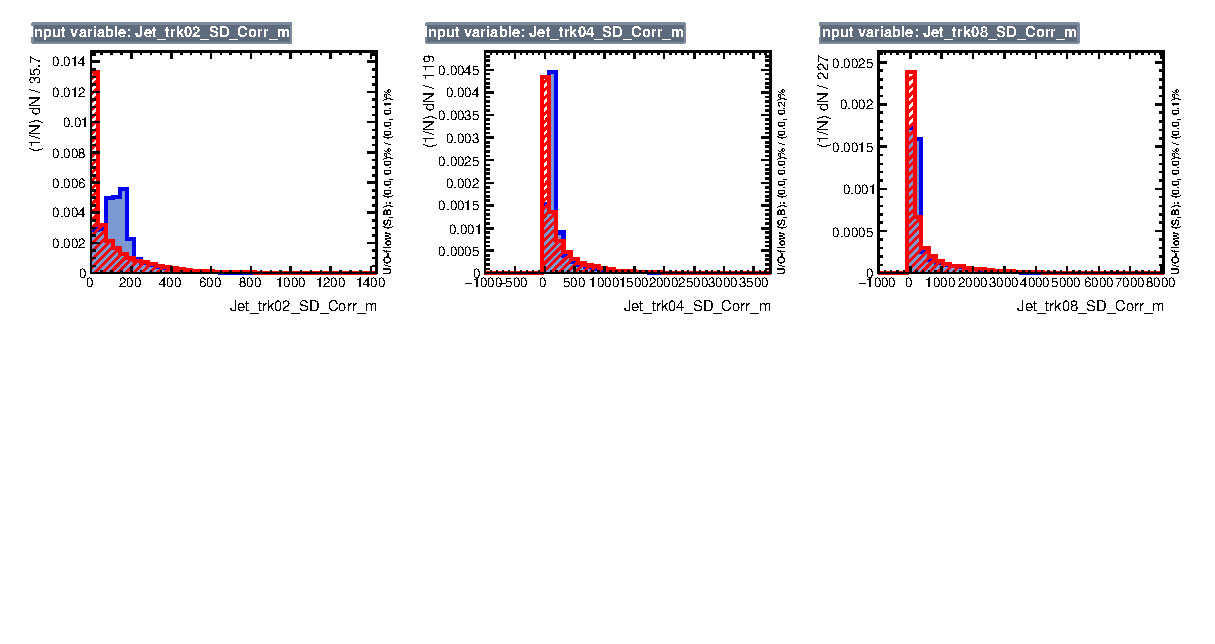
\includegraphics[width=0.495\textwidth]{Fig/TMVA/thad_vs_QCD/variables_id_c2.eps}
\caption{Input variables for top Vs QCD tagger.}
\label{fig:TMVA_inputs_t}
\end{figure}

\begin{figure}[!htb]\centering
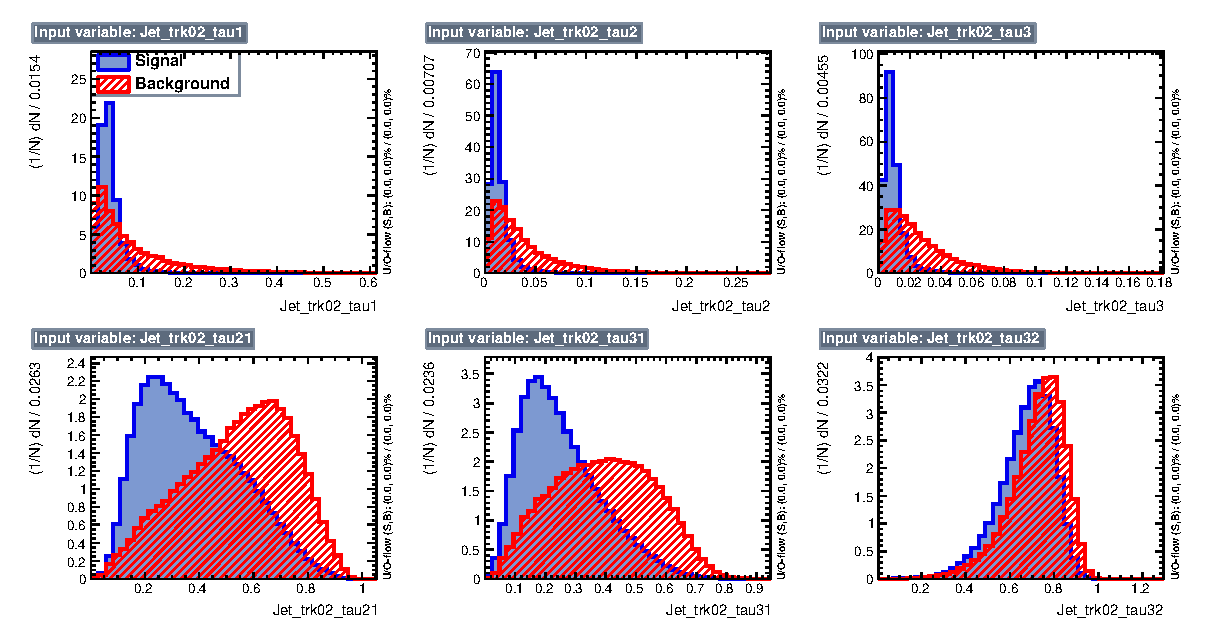
\includegraphics[width=0.495\textwidth]{Fig/TMVA/Whad_vs_QCD/variables_id_c1.eps}
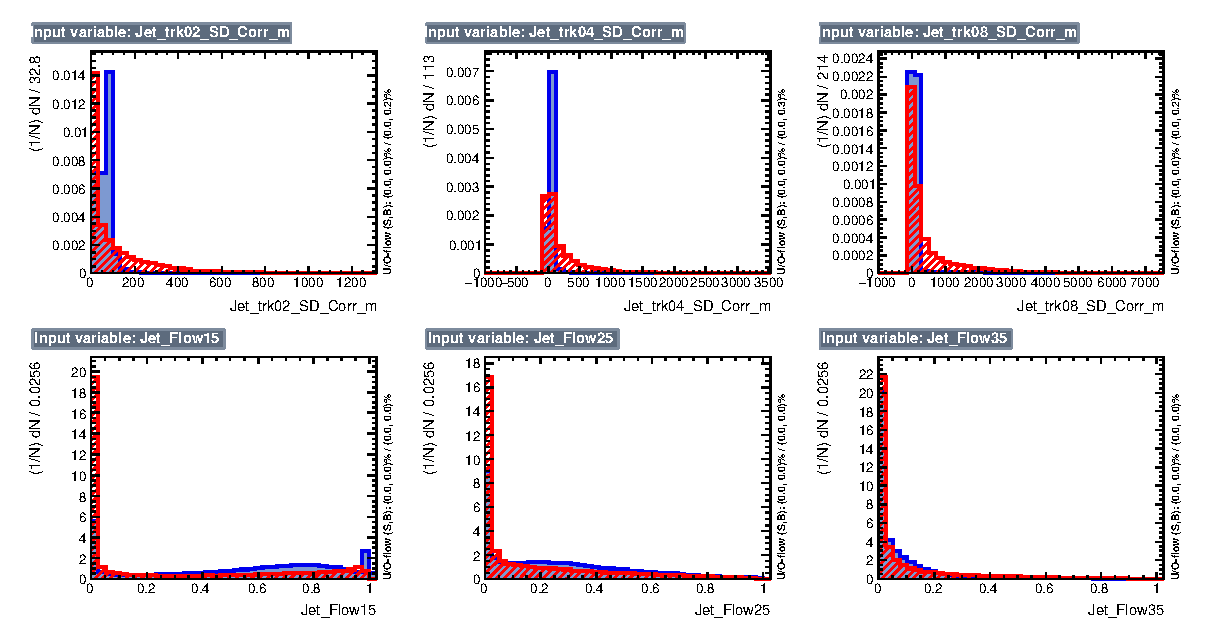
\includegraphics[width=0.495\textwidth]{Fig/TMVA/Whad_vs_QCD/variables_id_c2.eps}
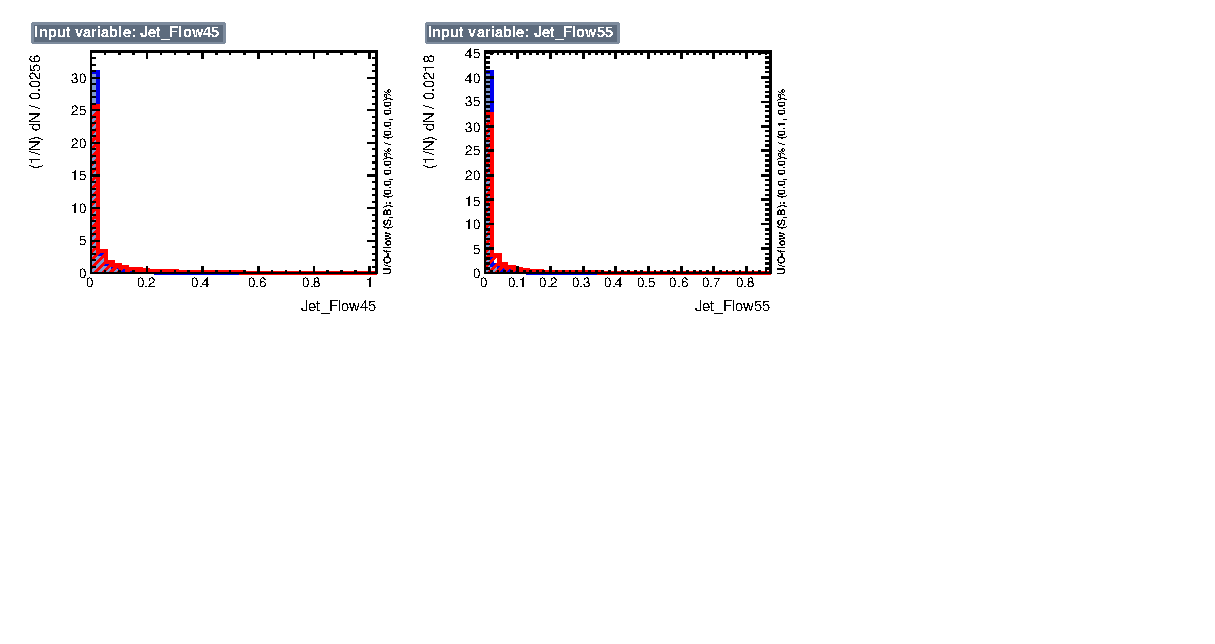
\includegraphics[width=0.495\textwidth]{Fig/TMVA/Whad_vs_QCD/variables_id_c3.eps}
\caption{Input variables for W Vs QCD tagger.}
\label{fig:TMVA_inputs_t}
\end{figure}

\begin{figure}[!htb]\centering
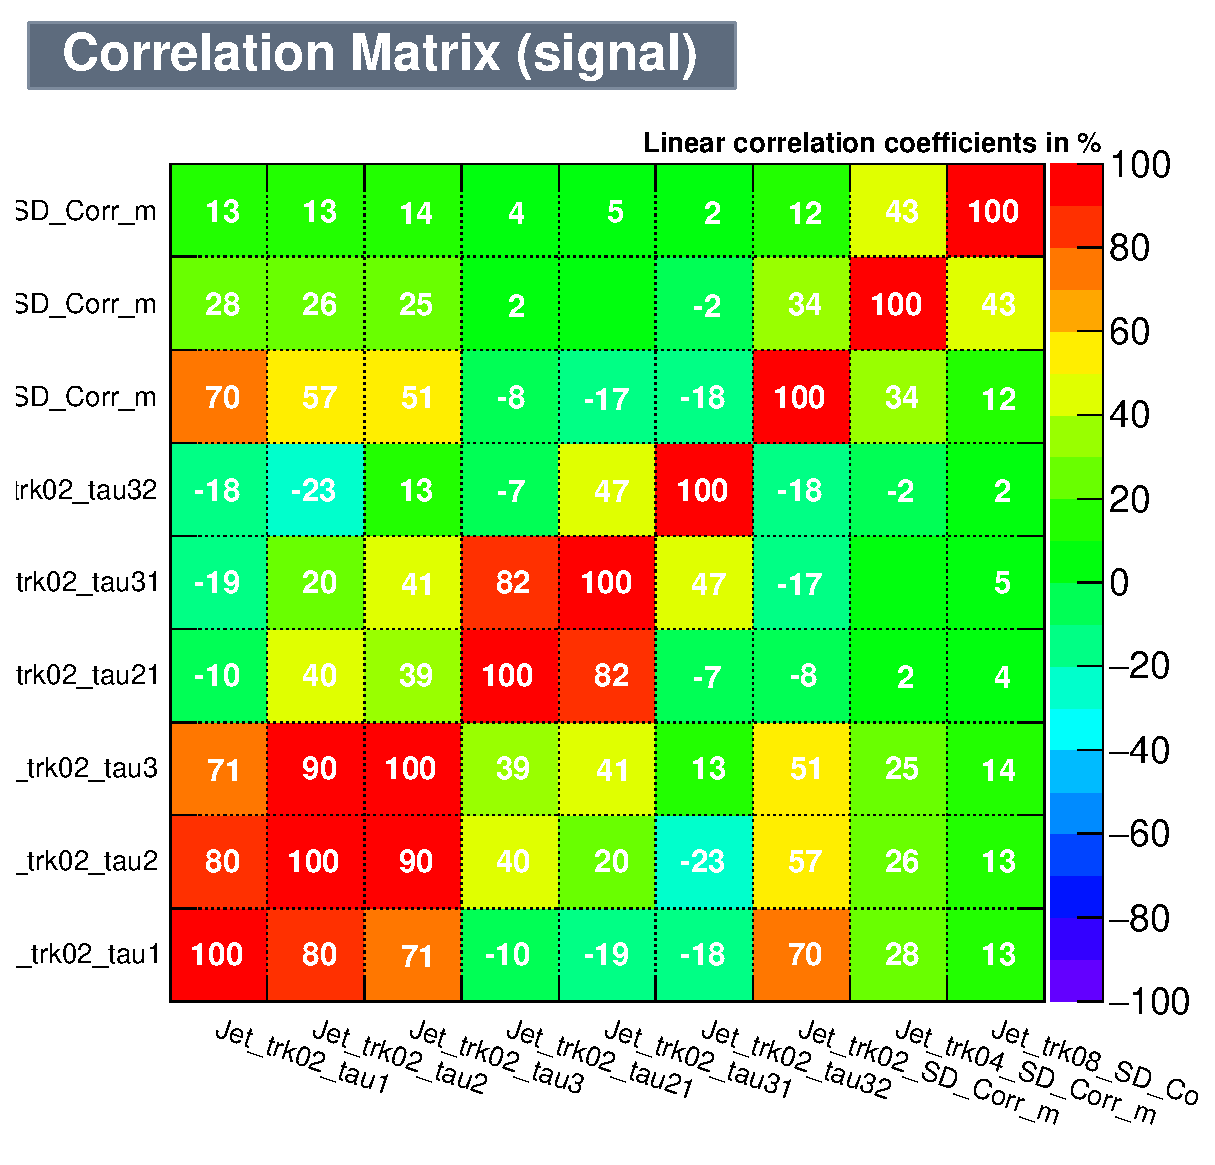
\includegraphics[width=0.495\textwidth]{Fig/TMVA/thad_vs_QCD/CorrelationMatrixS.eps}
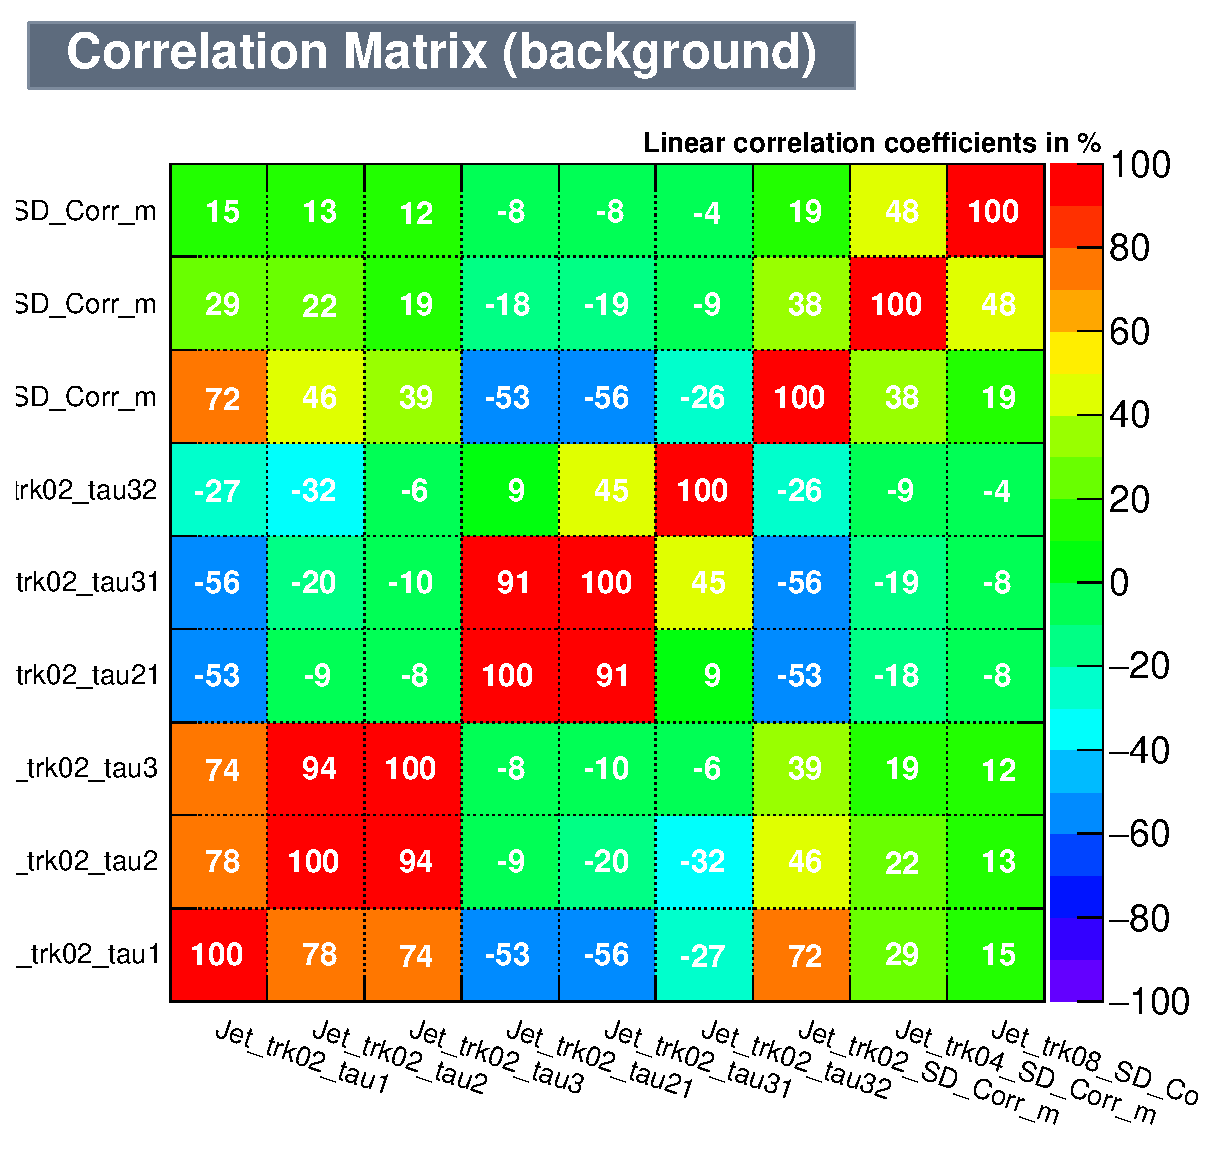
\includegraphics[width=0.495\textwidth]{Fig/TMVA/thad_vs_QCD/CorrelationMatrixB.eps}
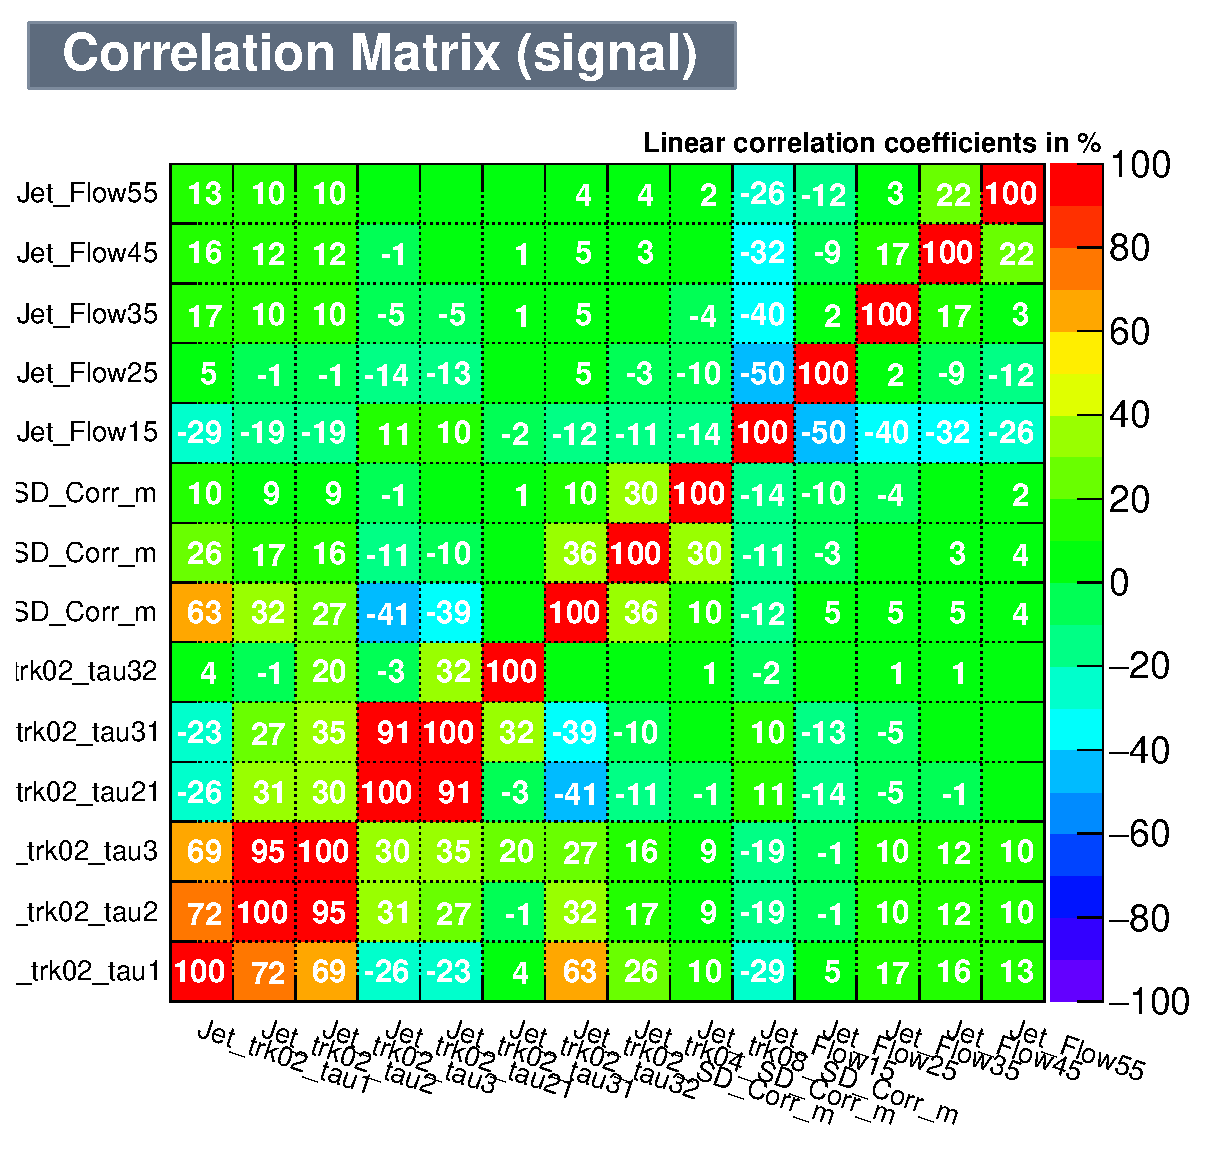
\includegraphics[width=0.495\textwidth]{Fig/TMVA/Whad_vs_QCD/CorrelationMatrixS.eps}
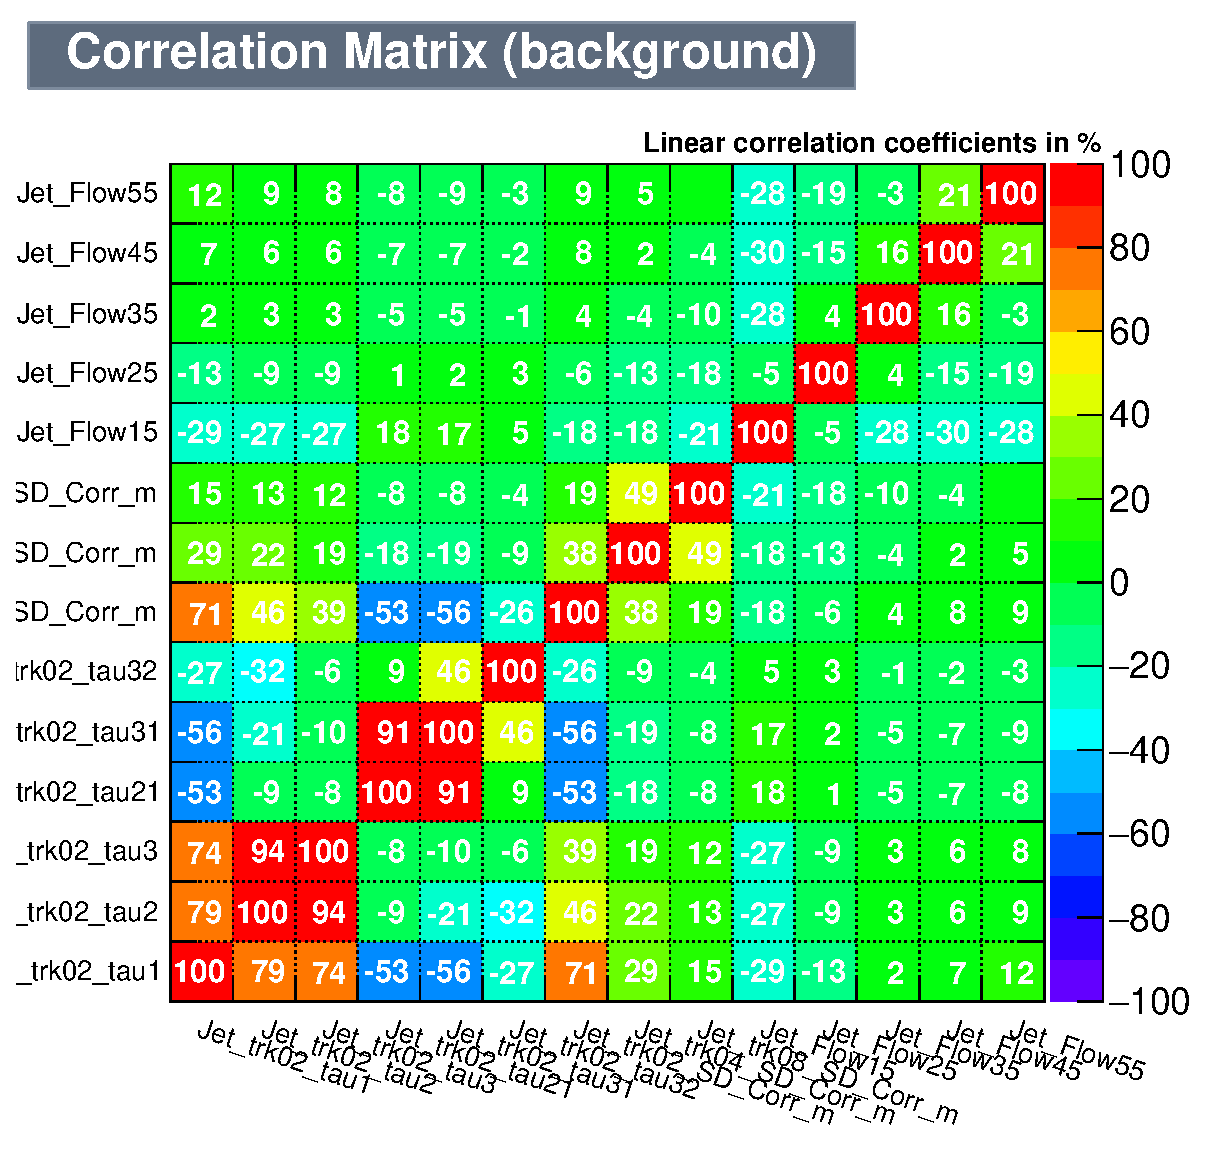
\includegraphics[width=0.495\textwidth]{Fig/TMVA/Whad_vs_QCD/CorrelationMatrixB.eps}
\caption{Correlation matrices for Signal (left) and Background (right) for top Vs QCD tagger (top) and W Vs QCD tagger (bottom).}
\label{fig:TMVA_corr_matrix}
\end{figure}

\begin{figure}[!htb]\centering
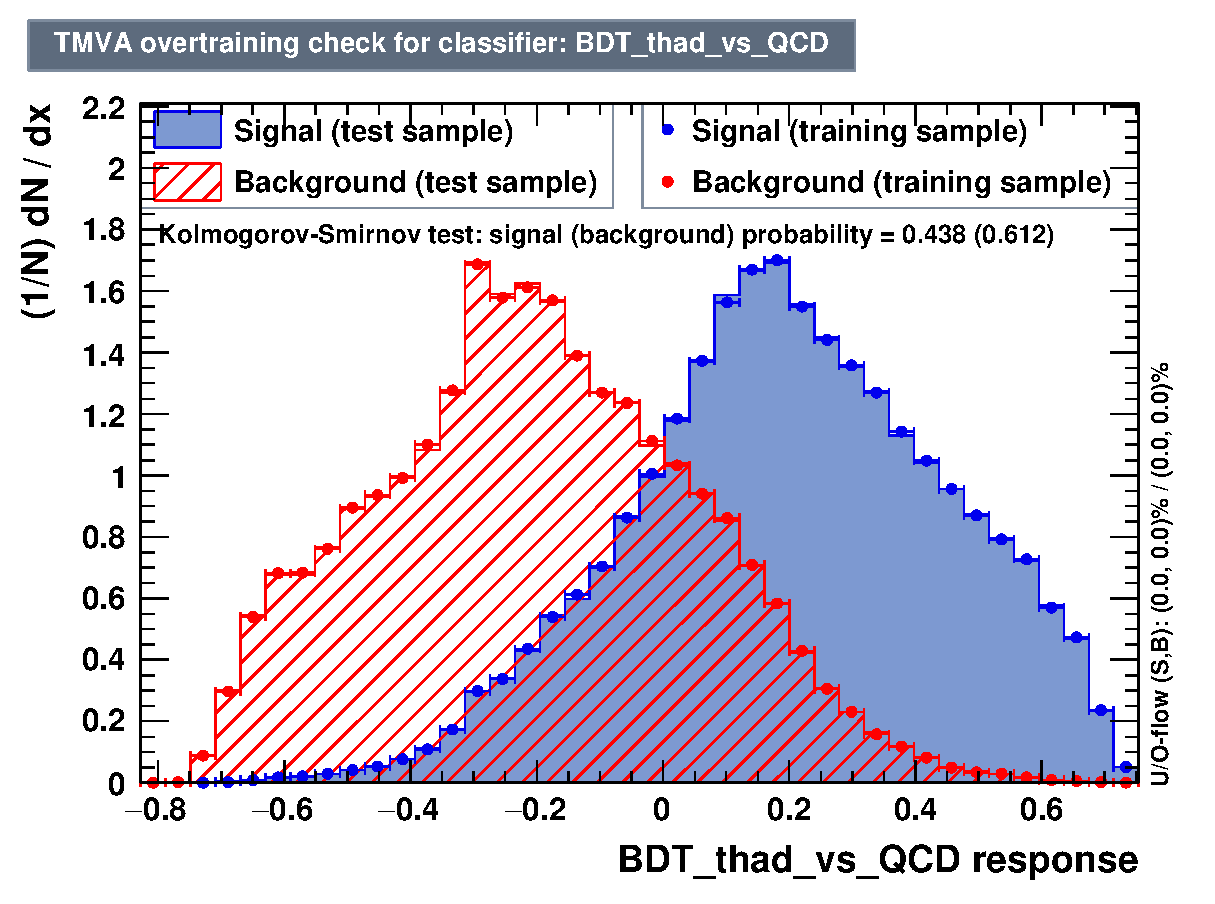
\includegraphics[width=0.495\textwidth]{Fig/TMVA/thad_vs_QCD/overtrain_BDT_thad_vs_QCD.eps}
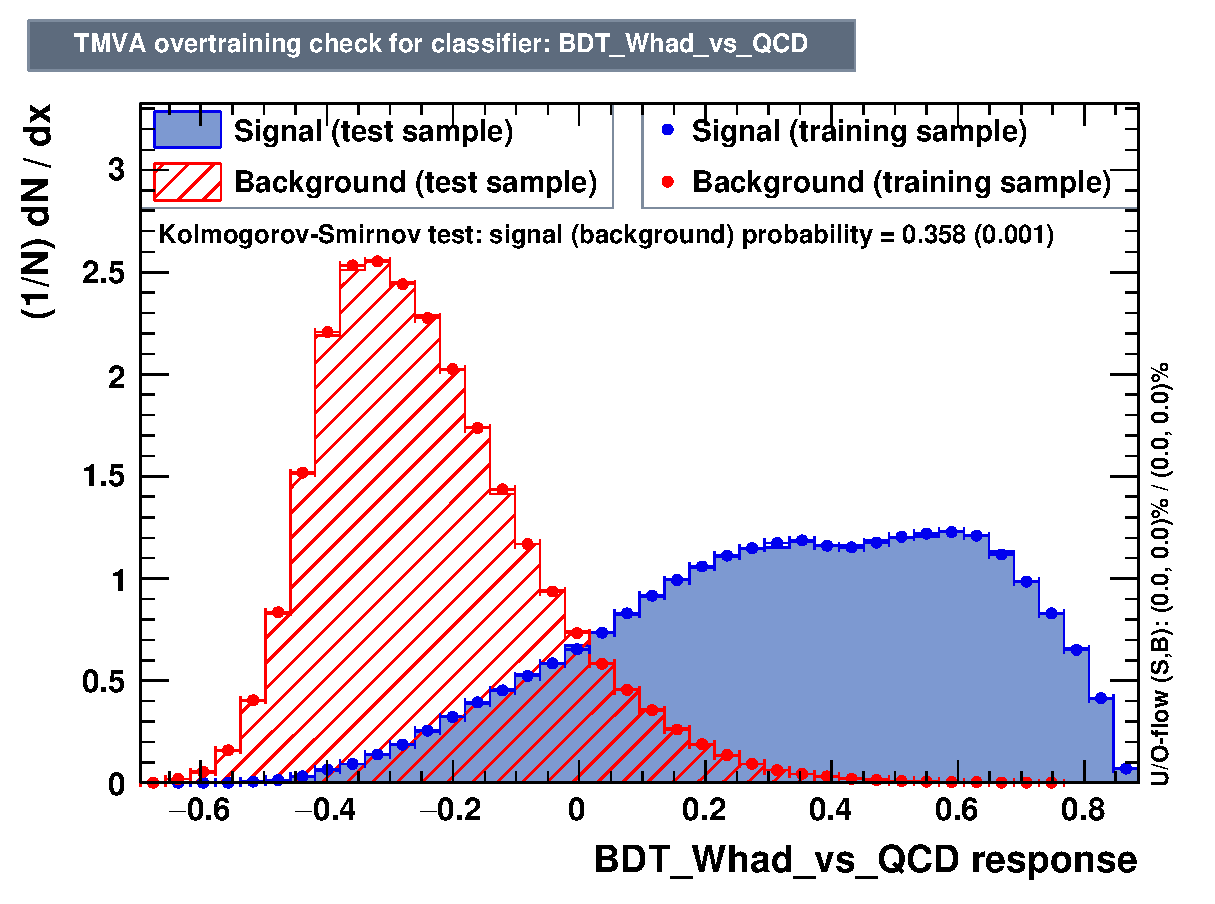
\includegraphics[width=0.495\textwidth]{Fig/TMVA/Whad_vs_QCD/overtrain_BDT_Whad_vs_QCD.eps}
\caption{BDT scores for Signal (red) and Background (blue) for top Vs QCD tagger (left) and W Vs QCD tagger (right).}
\label{fig:TMVA_BDTscore}
\end{figure}

\begin{figure}[!htb]\centering
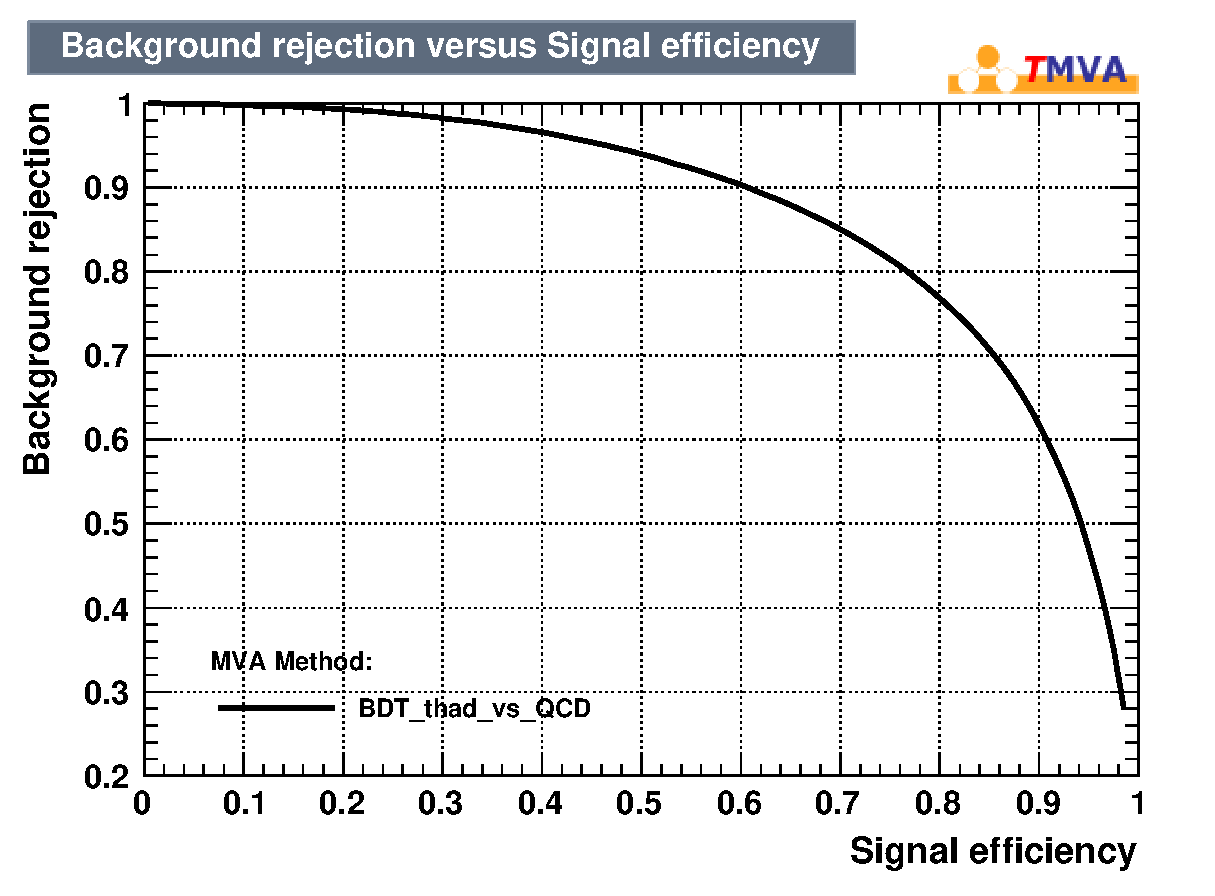
\includegraphics[width=0.495\textwidth]{Fig/TMVA/thad_vs_QCD/rejBvsS.eps}
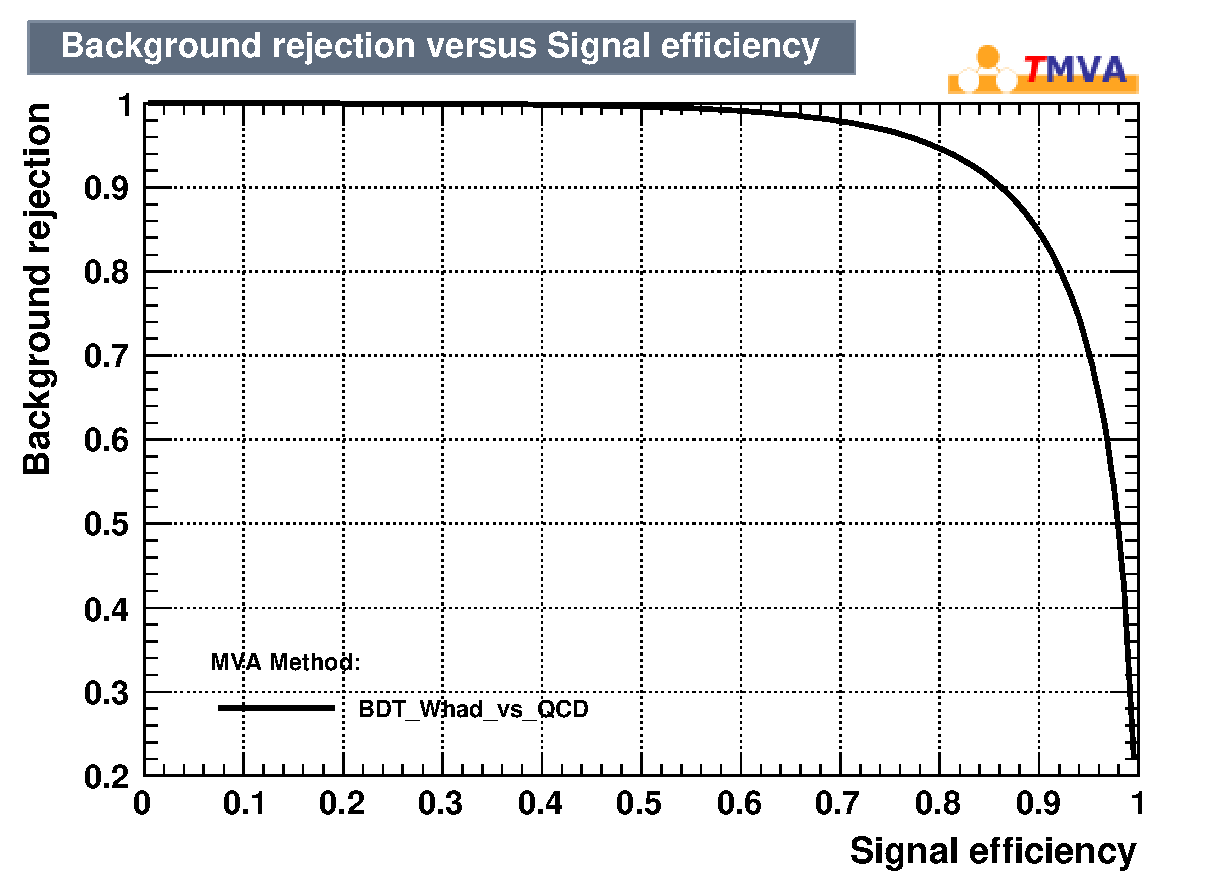
\includegraphics[width=0.495\textwidth]{Fig/TMVA/Whad_vs_QCD/rejBvsS.eps}
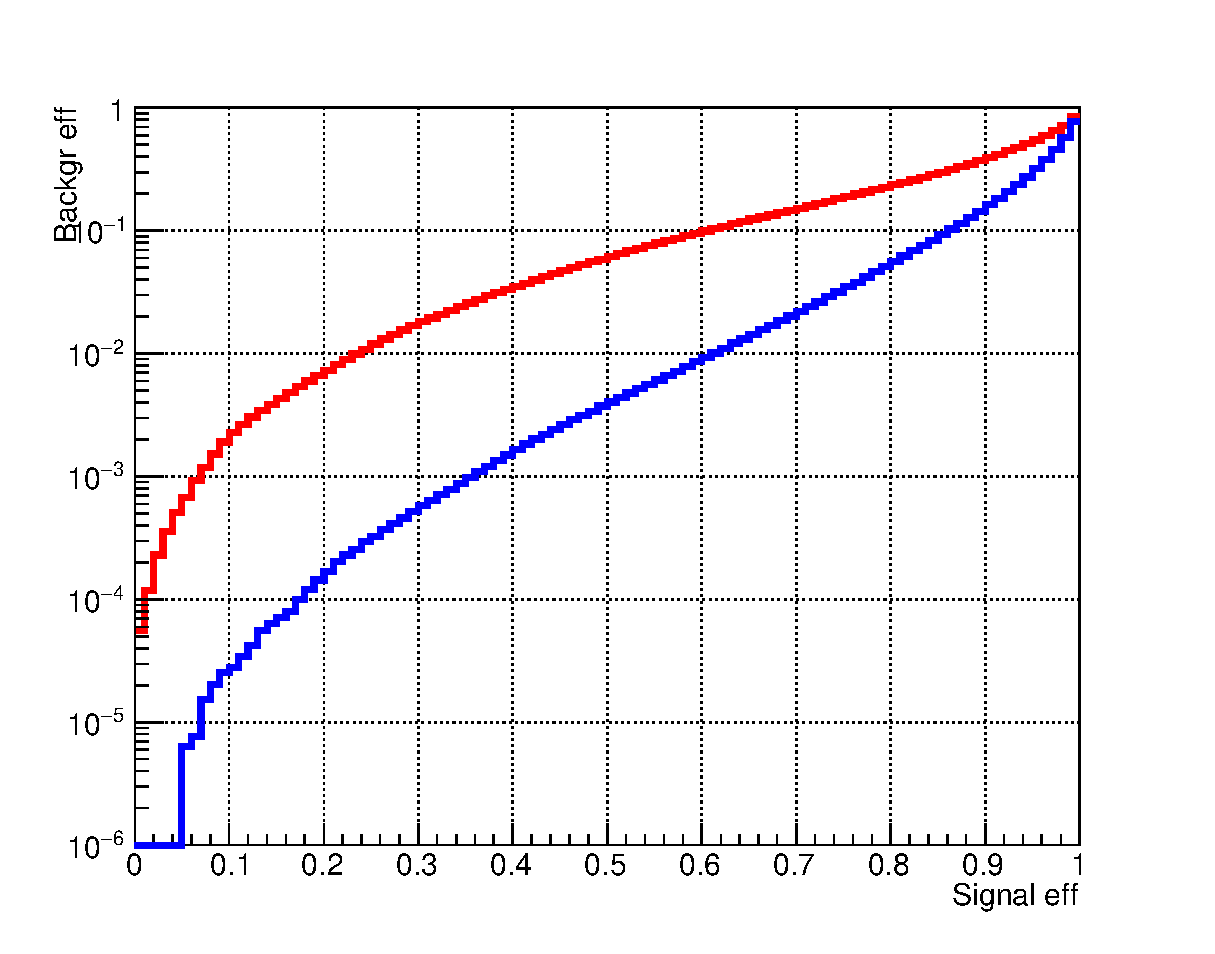
\includegraphics[width=0.495\textwidth]{Fig/TMVA/effQCD_vs_effWhadBlue_thadRed_log.eps}
\caption{Top ROC curves show background rejection Vs Signal efficiency for top Vs QCD tagger (left) and W Vs QCD tagger (right). Bottom ROC curves show background efficiency Vs signal efficiency overlay for top Vs QCD tagger (red) and W Vs QCD tagger (blue).}
\label{fig:TMVA_ROC}
\end{figure}

\begin{figure}[!htb]\centering
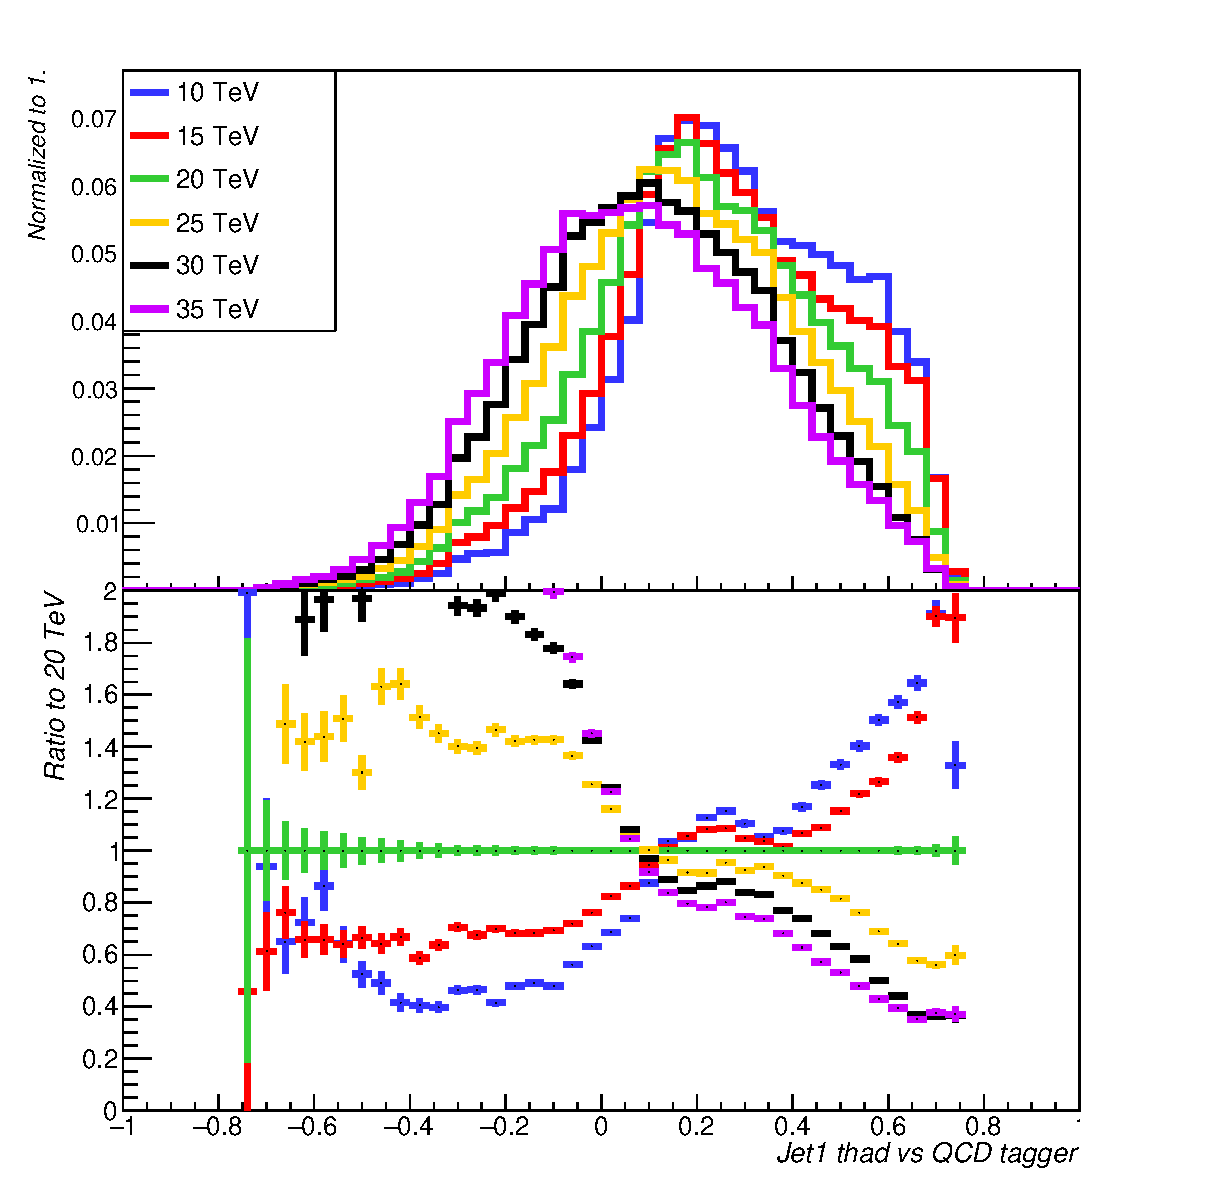
\includegraphics[width=0.495\textwidth]{Fig/TMVA/Jet1_thad_vs_QCD_tagger.eps}
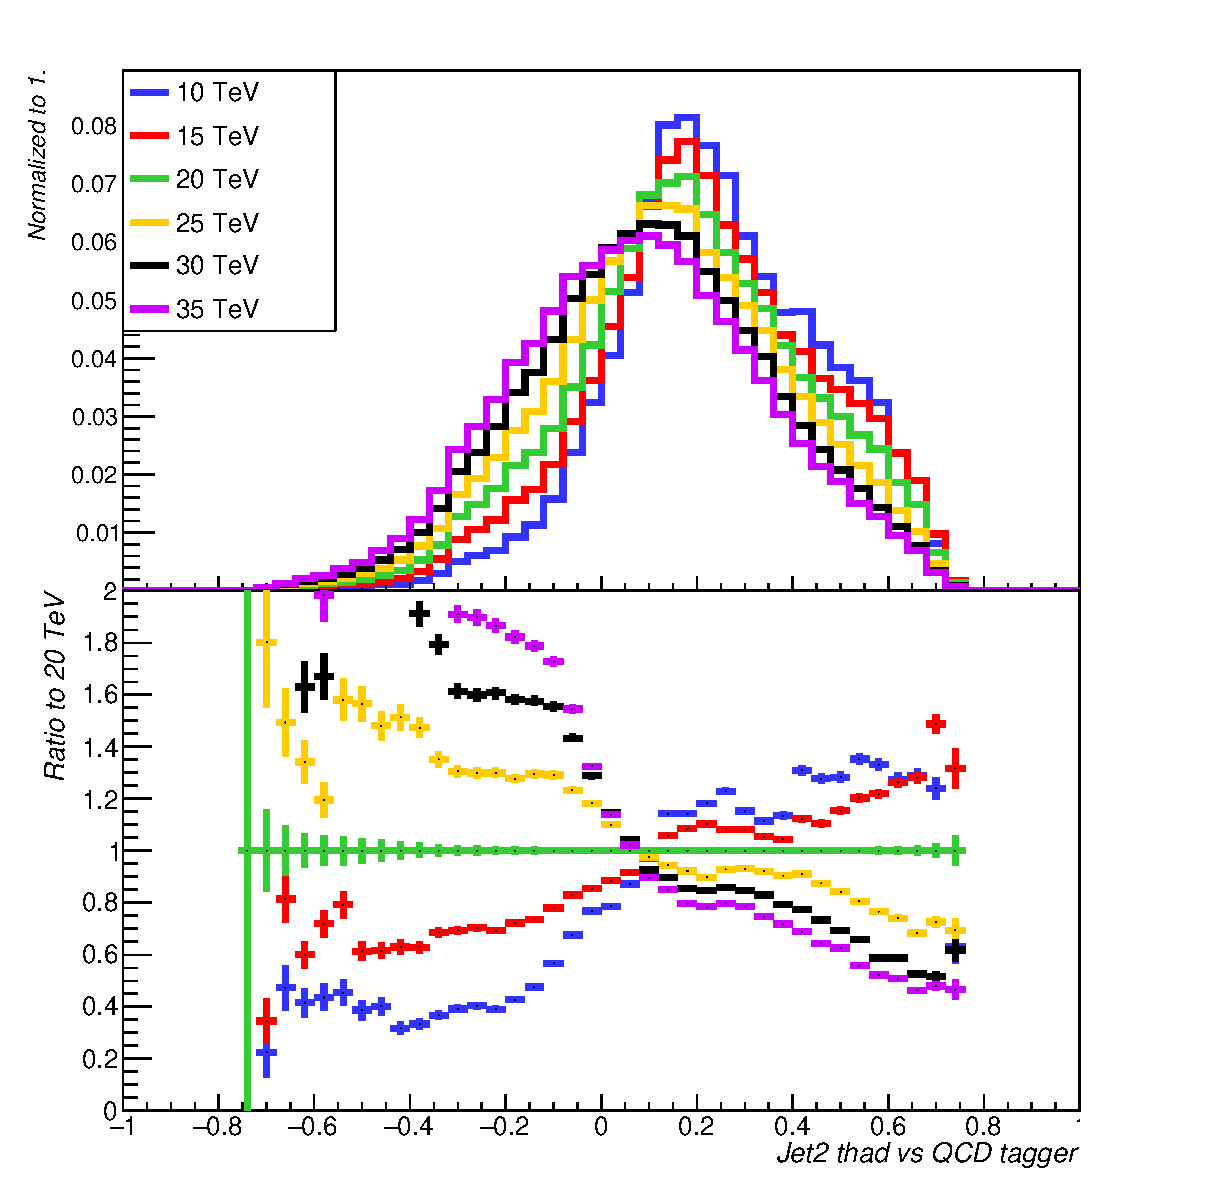
\includegraphics[width=0.495\textwidth]{Fig/TMVA/Jet2_thad_vs_QCD_tagger.eps}
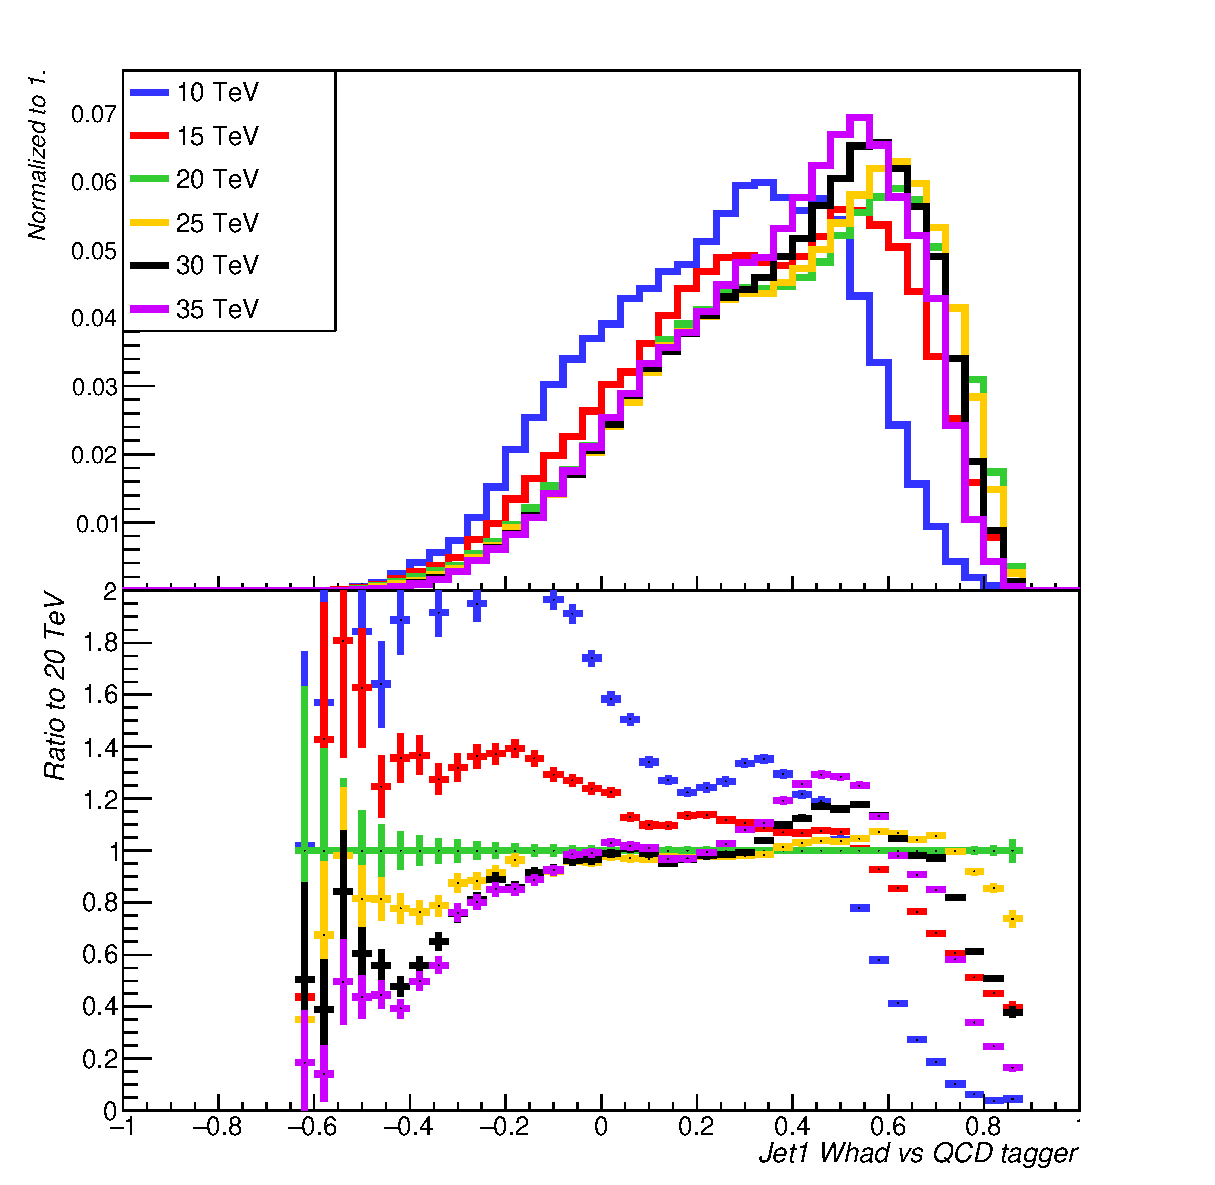
\includegraphics[width=0.495\textwidth]{Fig/TMVA/Jet1_Whad_vs_QCD_tagger.eps}
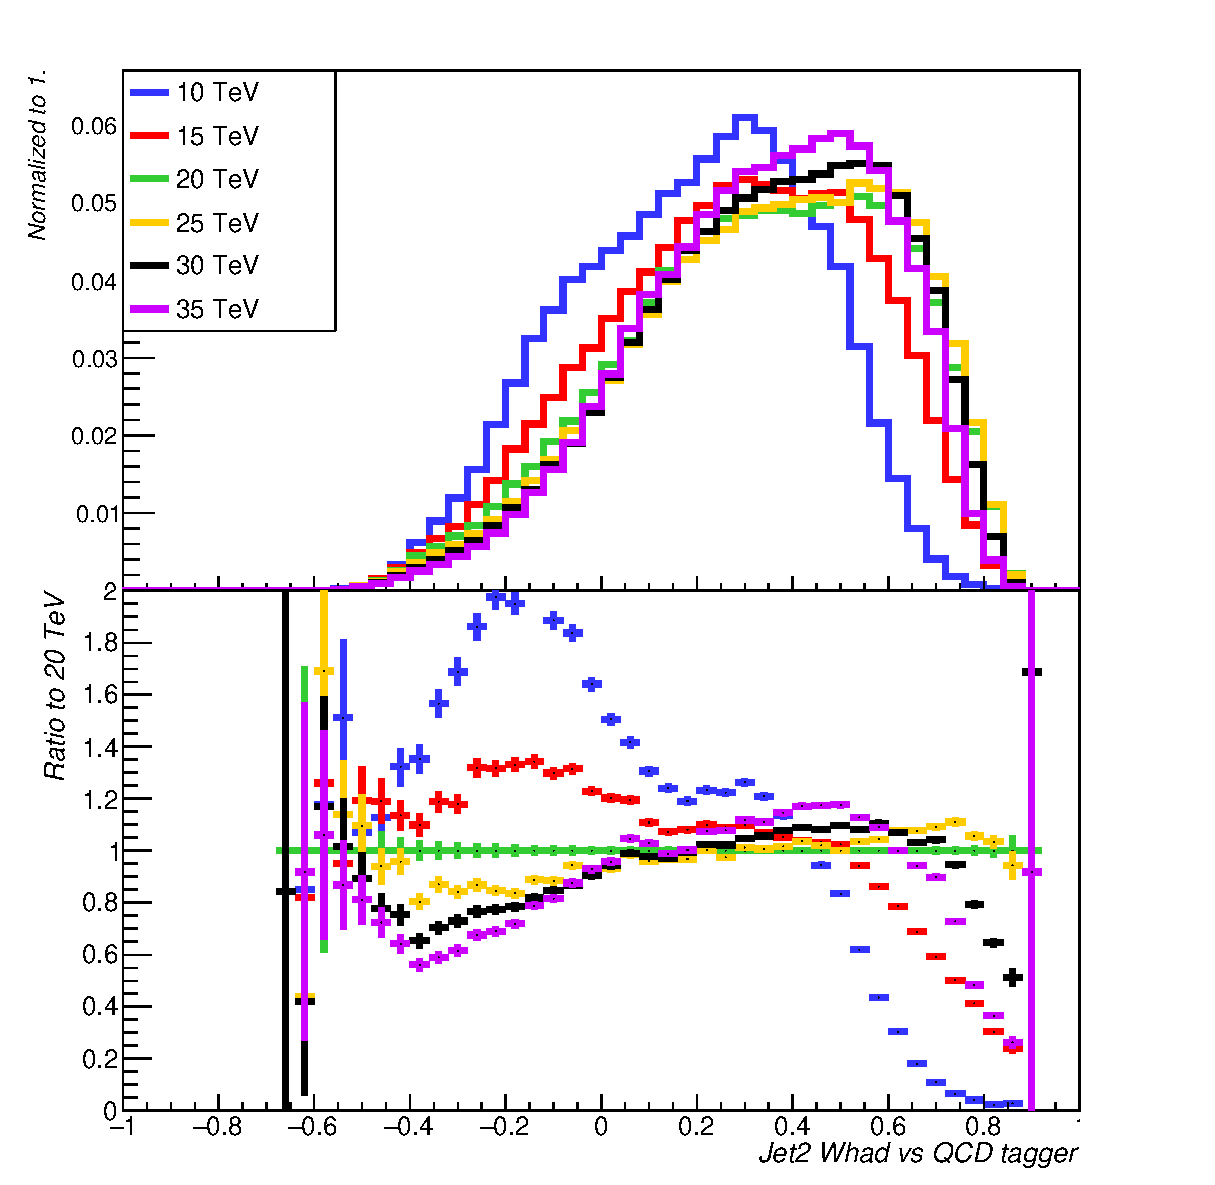
\includegraphics[width=0.495\textwidth]{Fig/TMVA/Jet2_Whad_vs_QCD_tagger.eps}
\caption{Signal BDT score shapes comparison for masses from 10 to 35 $\TeV$ (and ratio to 20 $\TeV$ mass) for leading jet (left) and second leading jet $\pt$ (right) for top Vs QCD tagger (top) and W Vs QCD tagger (bottom).}
\label{fig:BDT_signal_shape_comparison}
\end{figure}

\subsection{Limit settings}


\section{Physics models}

Models with extended gauge groups often feature additional U(1) symmetries with corresponding heavy spin-1 bosons. These bosons, generally referred to as $\Zp$, would manifest as a narrow resonance through
its  decay,  in  the  dilepton  mass  spectrum.   
Among  these  models  are  those  inspired  by  Grand  Unified Theories, which are 
motivated by gauge unification or a restoration of the left–right symmetry violated
by the weak interaction. Examples are the $\Zp$
bosons of the E6 motivated [1, 2] theories as well as Minimal models [3].  
The Sequential Standard Model (SSM) [2] posits a $\ZpSSM$ boson with couplings to fermions
that are identical to those of the SM $\Z$ boson. This model is a good benchmark as the 
results can be interpreted in the context of other models of new physics, and is useful 
for comparing the sensitivity of different experiments.



\section{Analyses}
\subsection{$\Zp \rightarrow ll$}
\begin{figure}[!htb]\centering
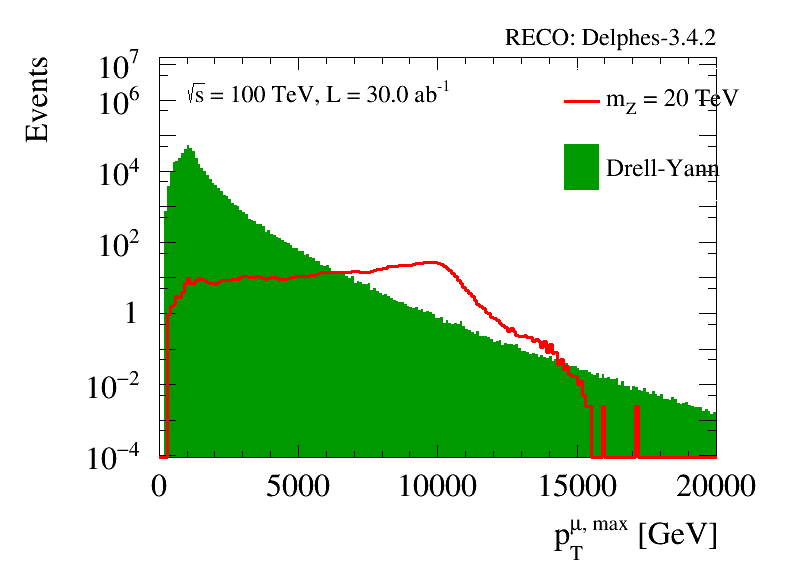
\includegraphics[width=0.495\textwidth]{Fig/FCC_ptmu_1_sel0_nostack_log.png}
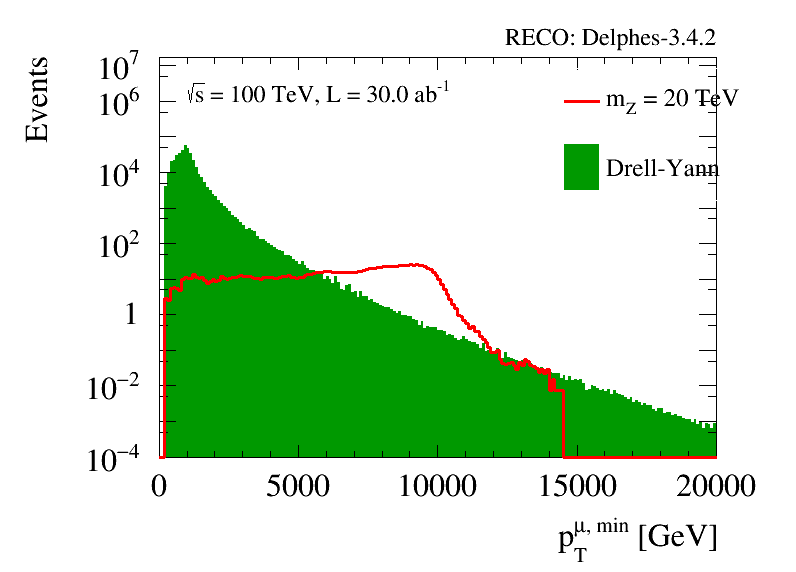
\includegraphics[width=0.495\textwidth]{Fig/FCC_ptmu_2_sel0_nostack_log.png}
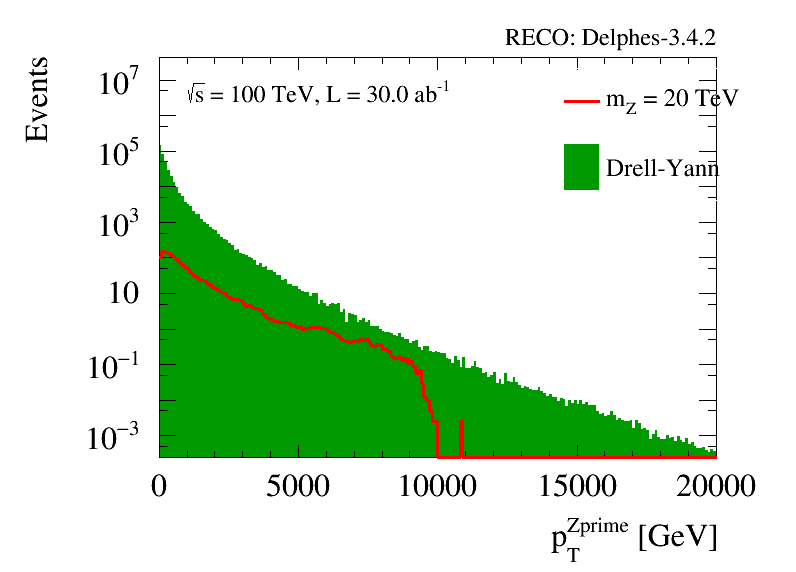
\includegraphics[width=0.495\textwidth]{Fig/FCC_ptzp_sel0_nostack_log.png}
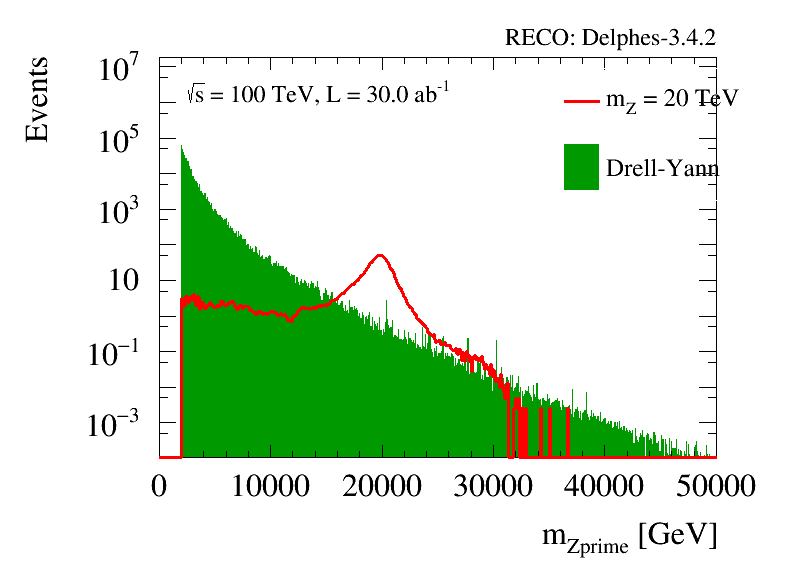
\includegraphics[width=0.495\textwidth]{Fig/FCC_mzp_sel0_nostack_log.png}
\caption{Leading (top left) and sub-leading (top right) $\ptMu$, $\ptZp$ (bottom left) and 
di-lepton invariant mass $\mll$ (bottom right) for the FCC 
baseline detector}
\label{fig:zpll_fcc}
\end{figure}


\begin{figure}[!htb]\centering
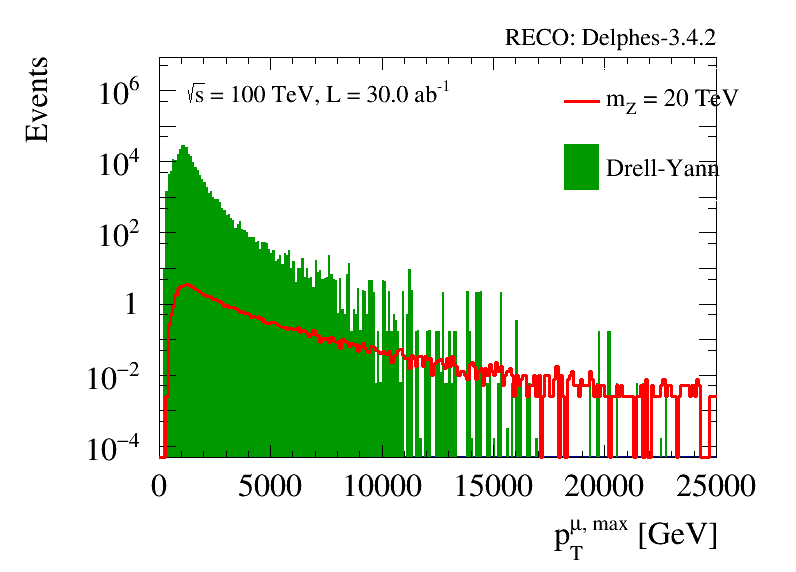
\includegraphics[width=0.495\textwidth]{Fig/CMS_ptmu_1_sel0_nostack_log.png}
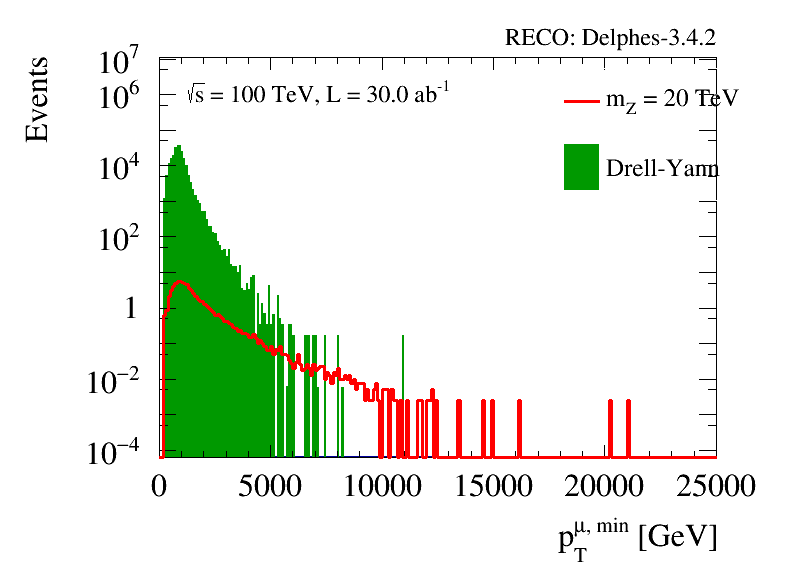
\includegraphics[width=0.495\textwidth]{Fig/CMS_ptmu_2_sel0_nostack_log.png}
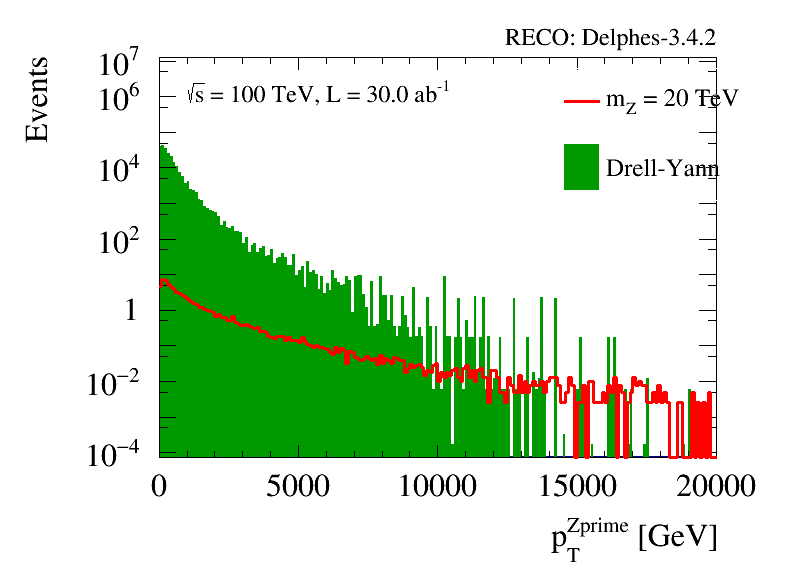
\includegraphics[width=0.495\textwidth]{Fig/CMS_ptzp_sel0_nostack_log.png}
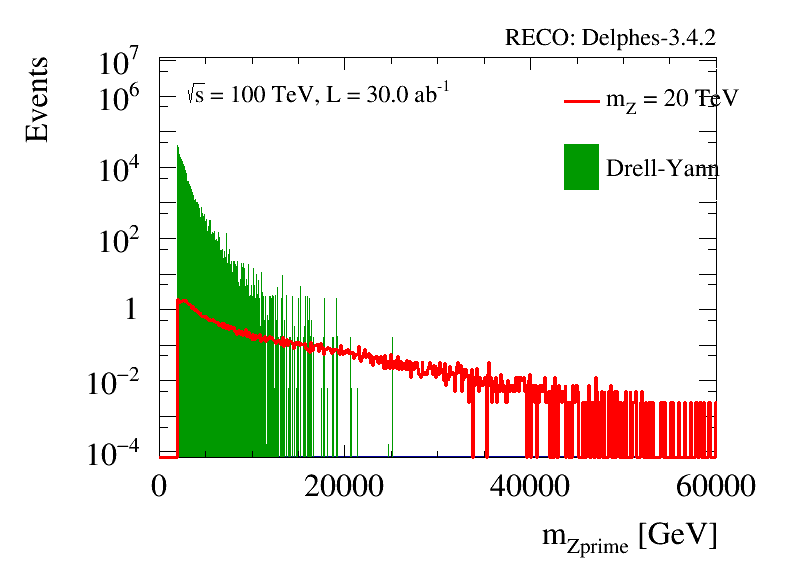
\includegraphics[width=0.495\textwidth]{Fig/CMS_mzp_sel0_nostack_log.png}
\caption{Leading (top left) and sub-leading (top right) $\ptMu$, $\ptZp$ (bottom left) and 
di-lepton invariant mass $\mll$ (bottom right) for the CMS  detector}
\label{fig:zpll_cms}
\end{figure}

\begin{figure}[!htb]\centering
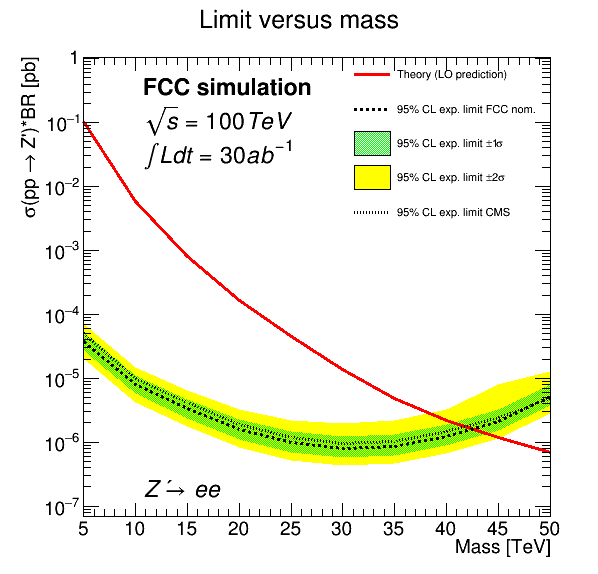
\includegraphics[width=0.495\textwidth]{Fig/lim_Zprime_ee_fcc_cms.png}
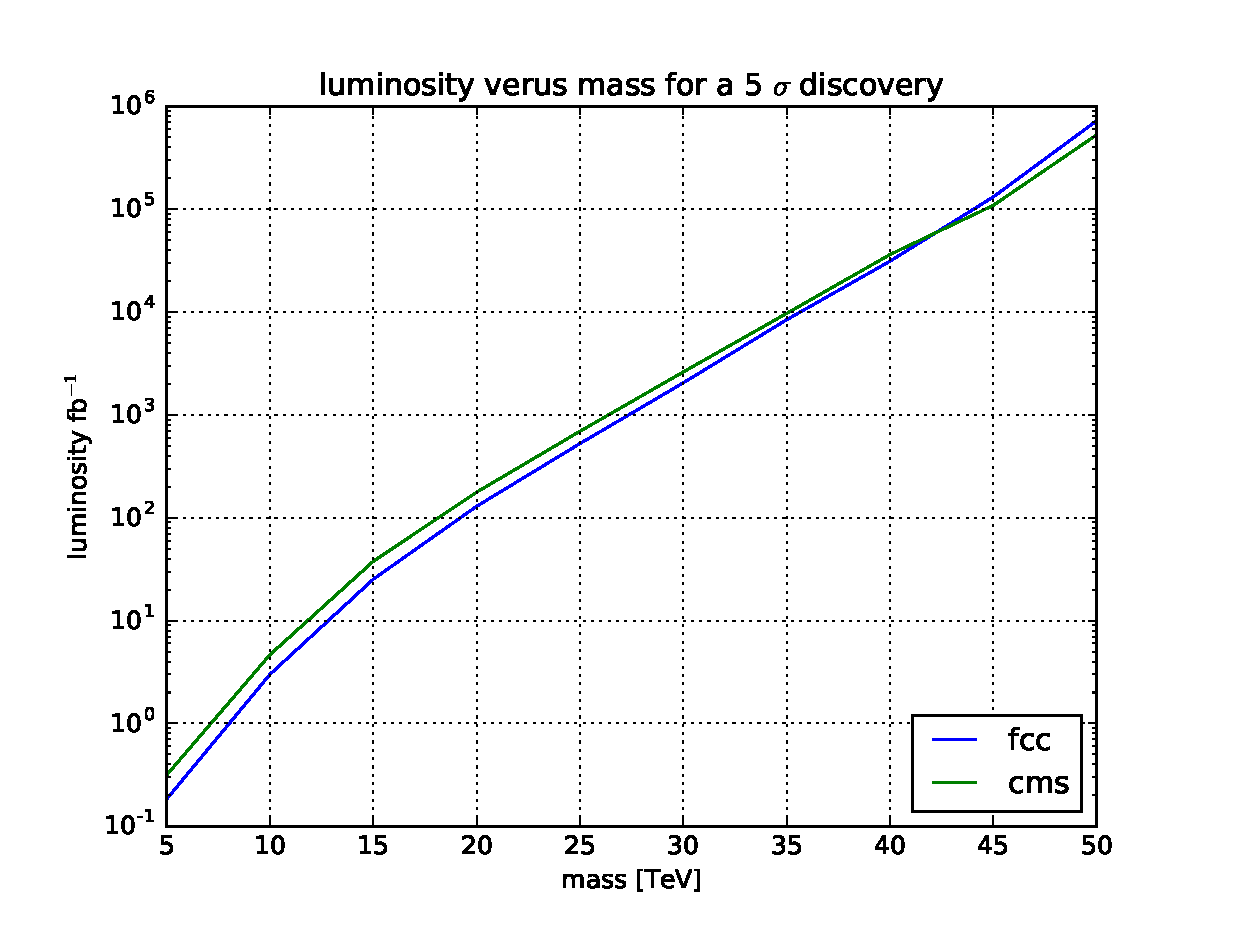
\includegraphics[width=0.495\textwidth]{Fig/DiscoveryPotential_ee.eps}
\caption{Limit versus mass (left) and luminosity for a $5\sigma$ discovery (right) for the
 di-electron channel.}
\label{fig:zpee_lim}
\end{figure}

\begin{figure}[!htb]\centering
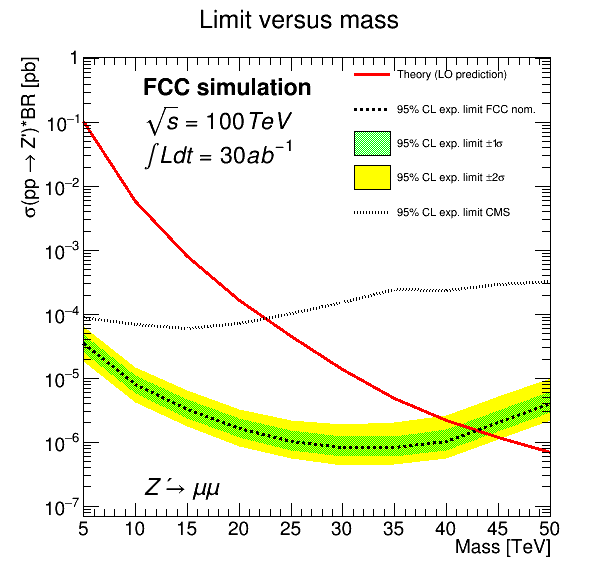
\includegraphics[width=0.495\textwidth]{Fig/lim_Zprime_mumu_fcc_cms.png}
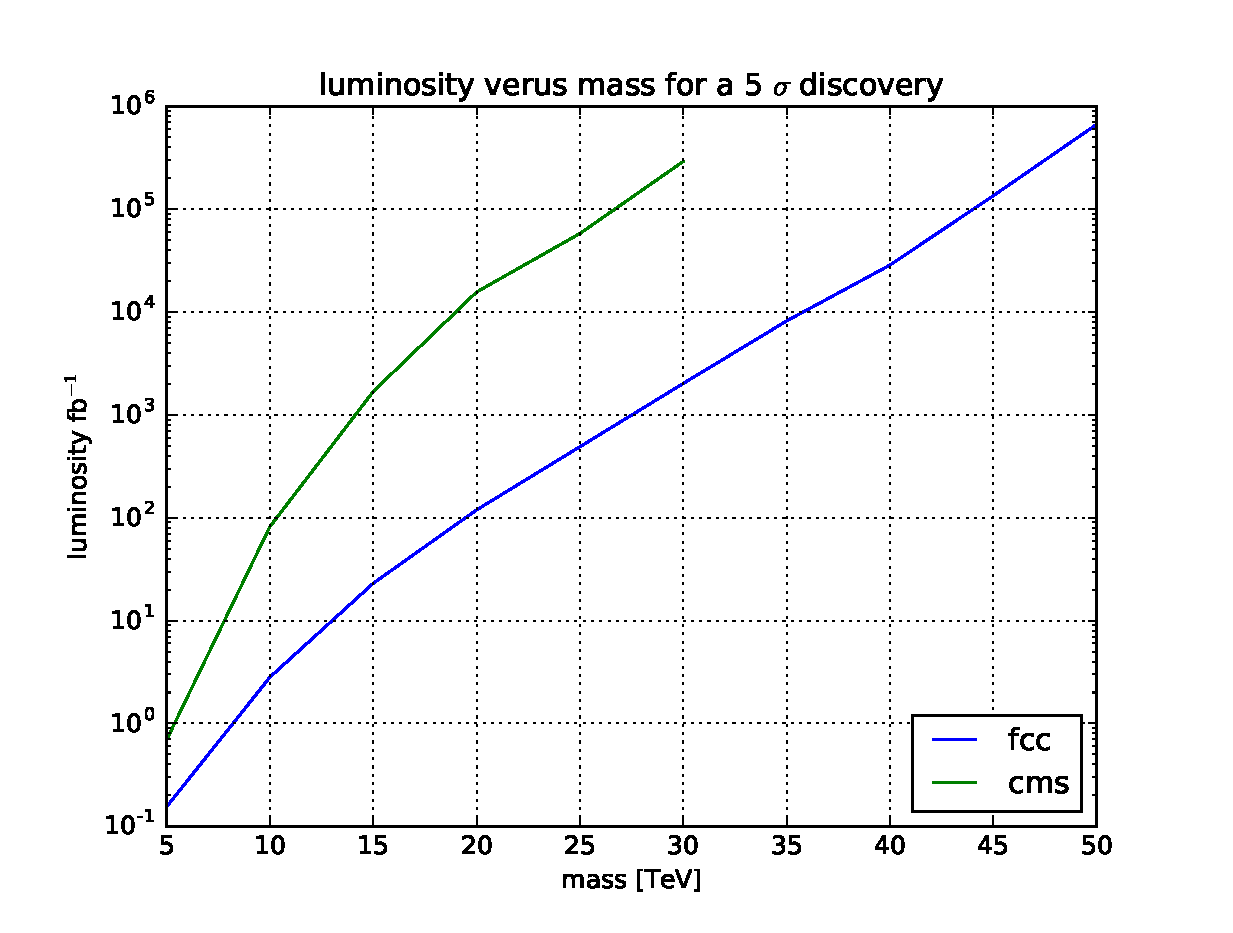
\includegraphics[width=0.495\textwidth]{Fig/DiscoveryPotential_mumu.eps}
\caption{Limit versus mass (left) and luminosity for a $5\sigma$ discovery (right) for the
 di-muon channel.}
\label{fig:zpmumu_lim}
\end{figure}

\begin{figure}[!htb]\centering
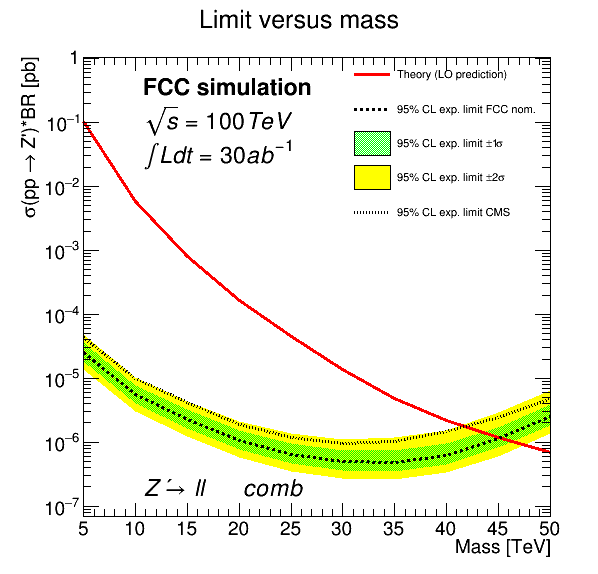
\includegraphics[width=0.495\textwidth]{Fig/lim_Zprime_ll_fcc_cms.png}
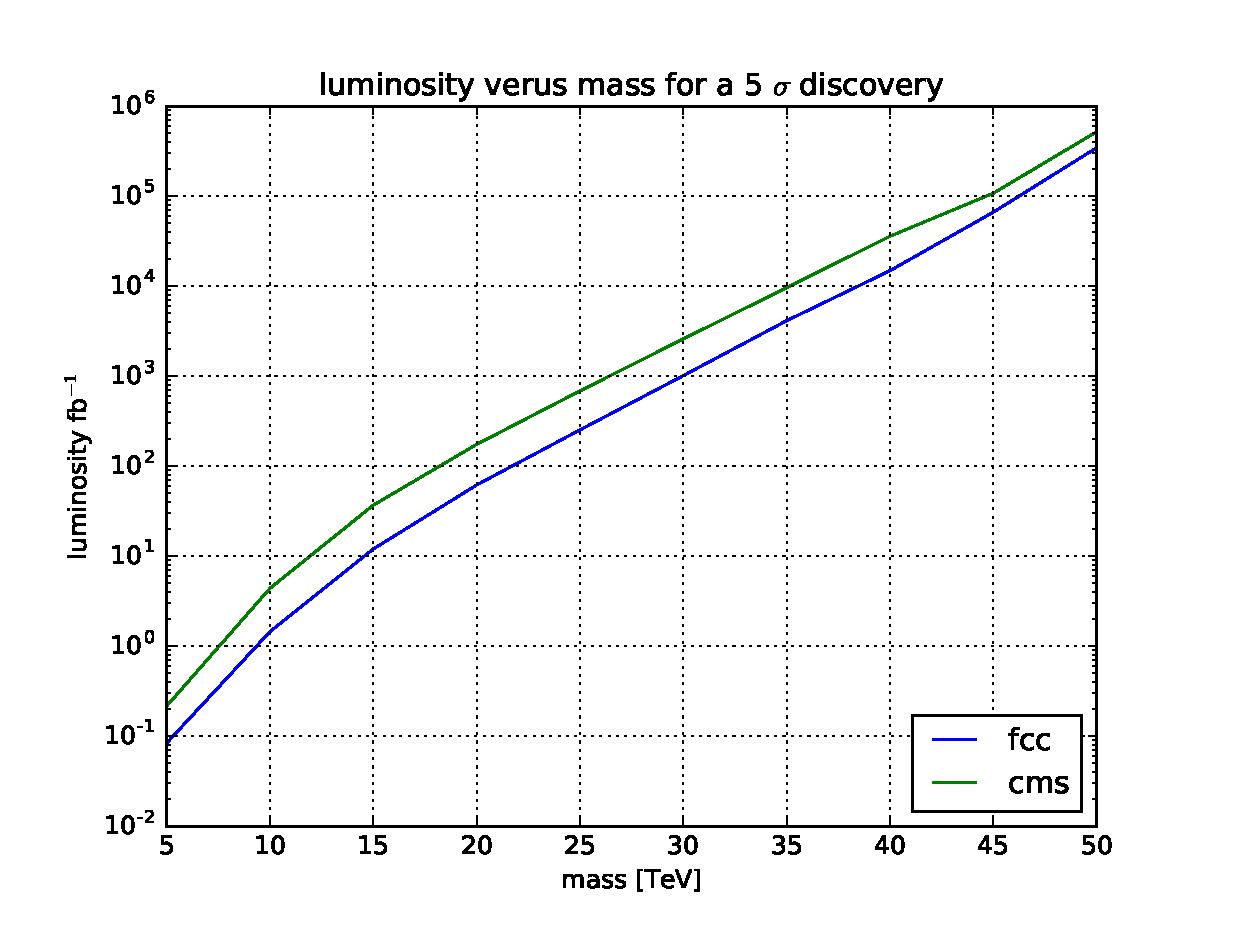
\includegraphics[width=0.495\textwidth]{Fig/DiscoveryPotential_ll.eps}
\caption{Limit versus mass (left) and luminosity for a $5\sigma$ discovery (right) for the
 di-lepton channel combined.}
\label{fig:zpll_lim}
\end{figure}

\subsection{$\Zp \rightarrow \ttbar$}
\label{subsec:Zptt}

Backgrounds: QCD, ttbar, single top, V+jets, VV. 

\begin{figure}[!htb]\centering
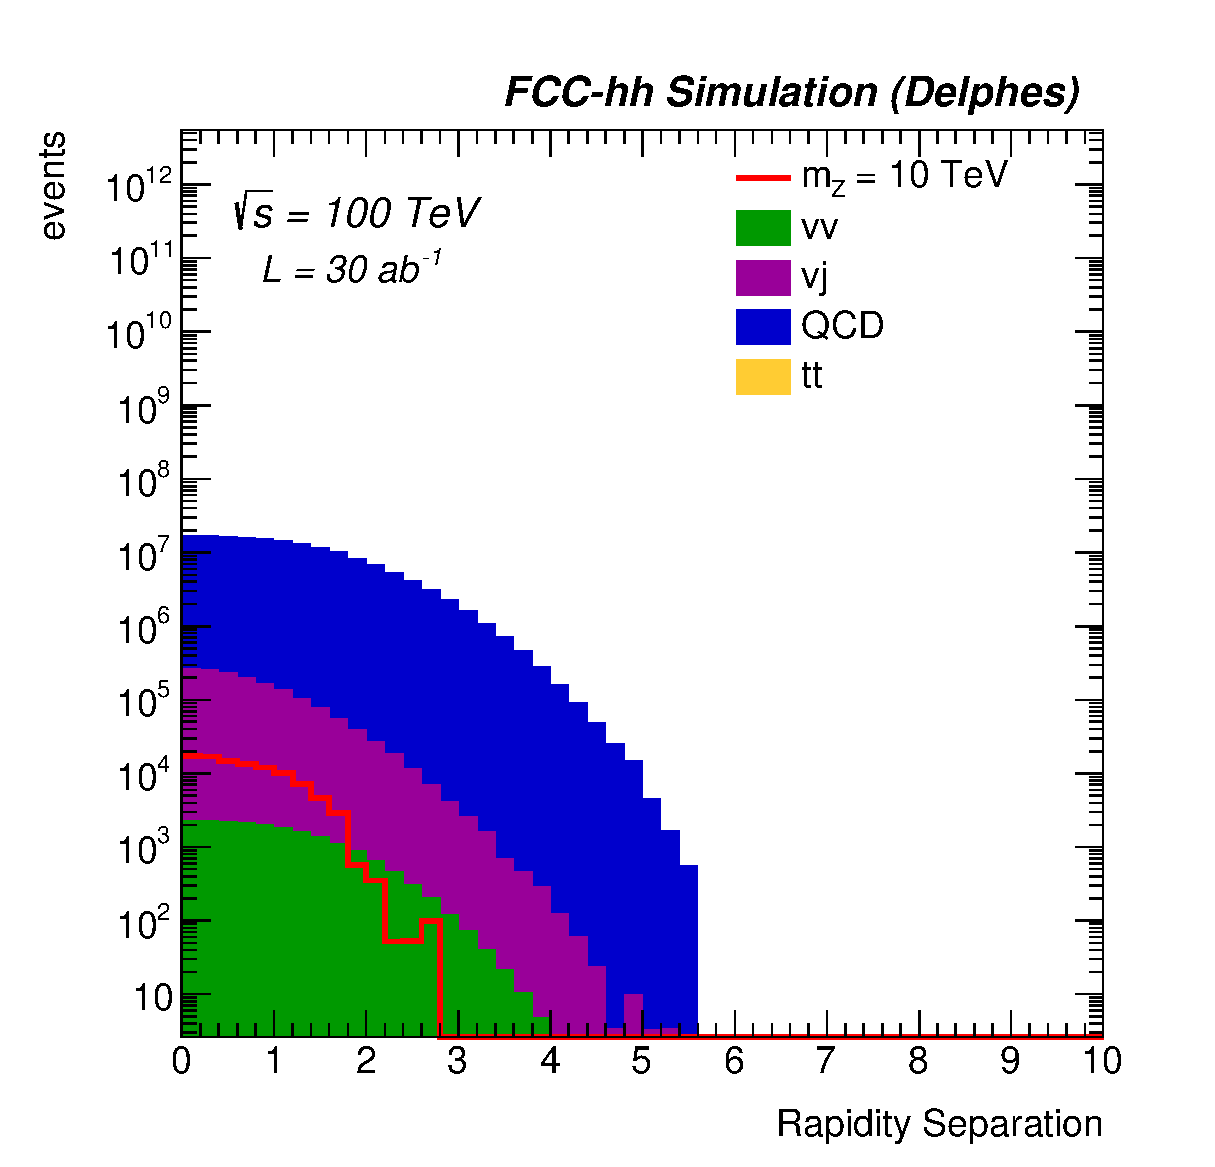
\includegraphics[width=0.8\textwidth]{Fig/Zptt/rapiditySeparation_sel0_before_cut_nostack_log.eps}
\caption{Rapidity separation at preselection level before cut on this variable in $\Zp \rightarrow \ttbar$ analysis. The generated mass of the signal sample is 10 $\TeV$.}
\label{fig:Zptt_sel0_rapidity}
\end{figure}

\begin{figure}[!htb]\centering
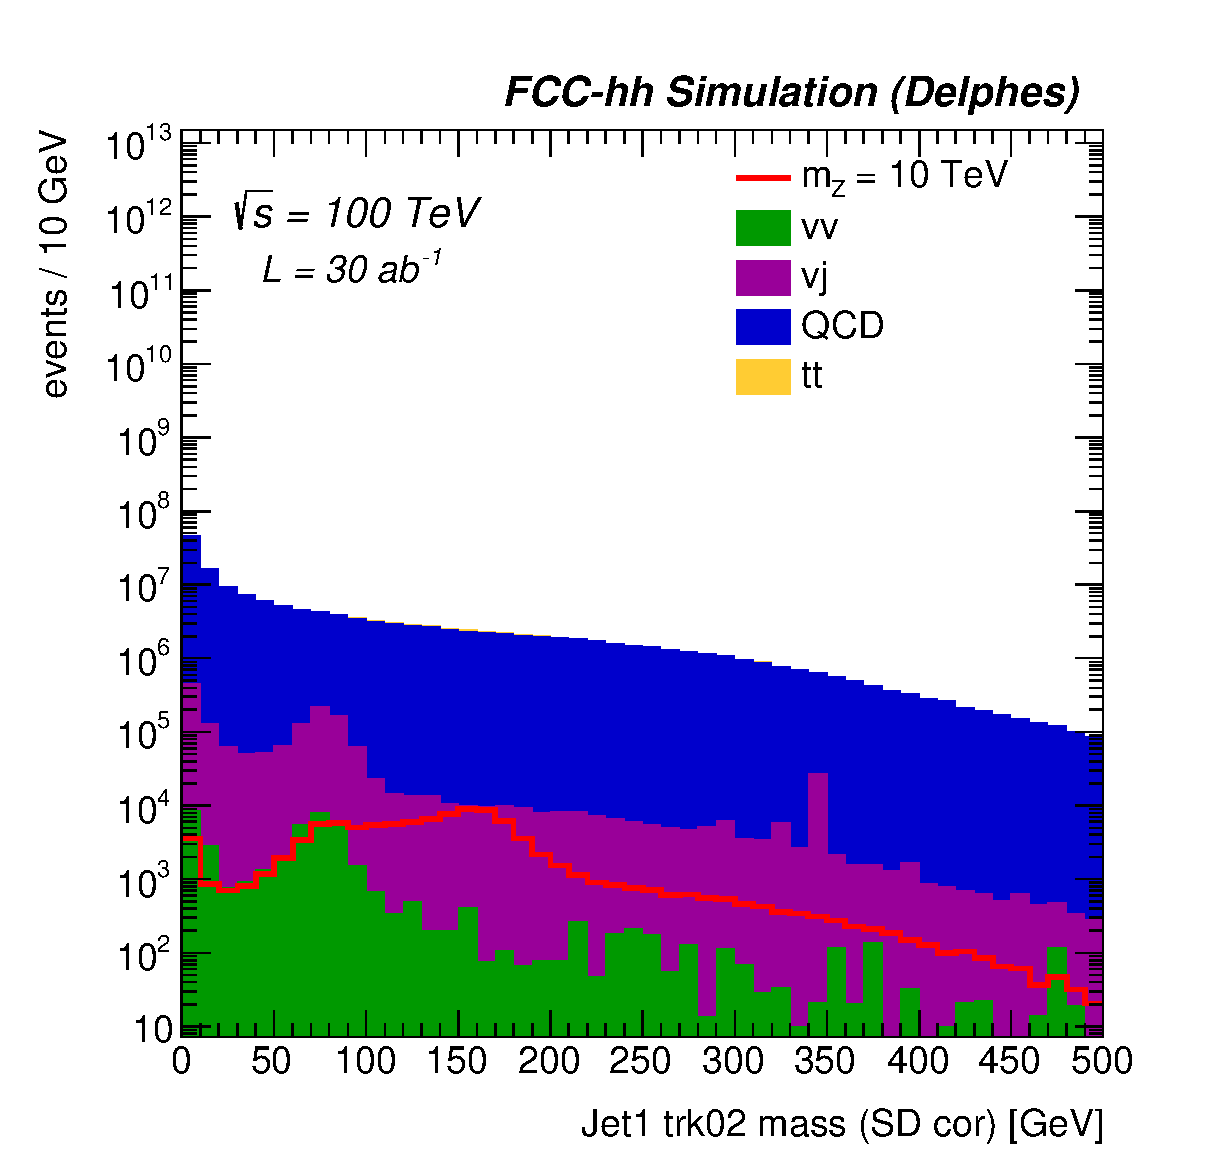
\includegraphics[width=0.495\textwidth]{Fig/Zptt/Jet1_trk02_SD_Cor_m_sel0_nostack_log.eps}
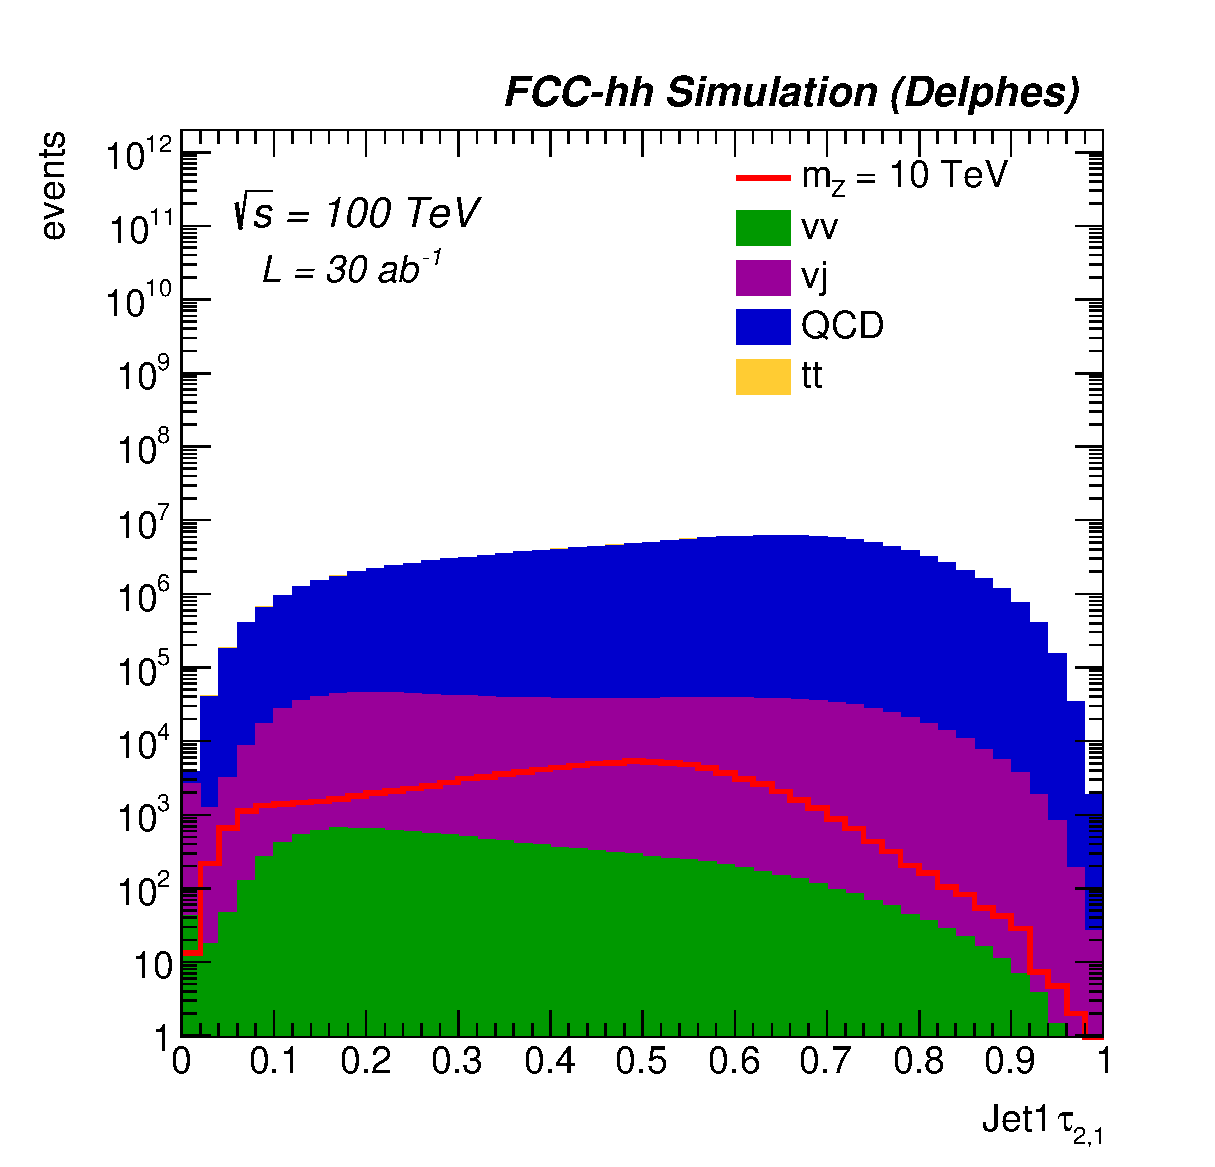
\includegraphics[width=0.495\textwidth]{Fig/Zptt/Jet1_tau21_sel0_nostack_log.eps}
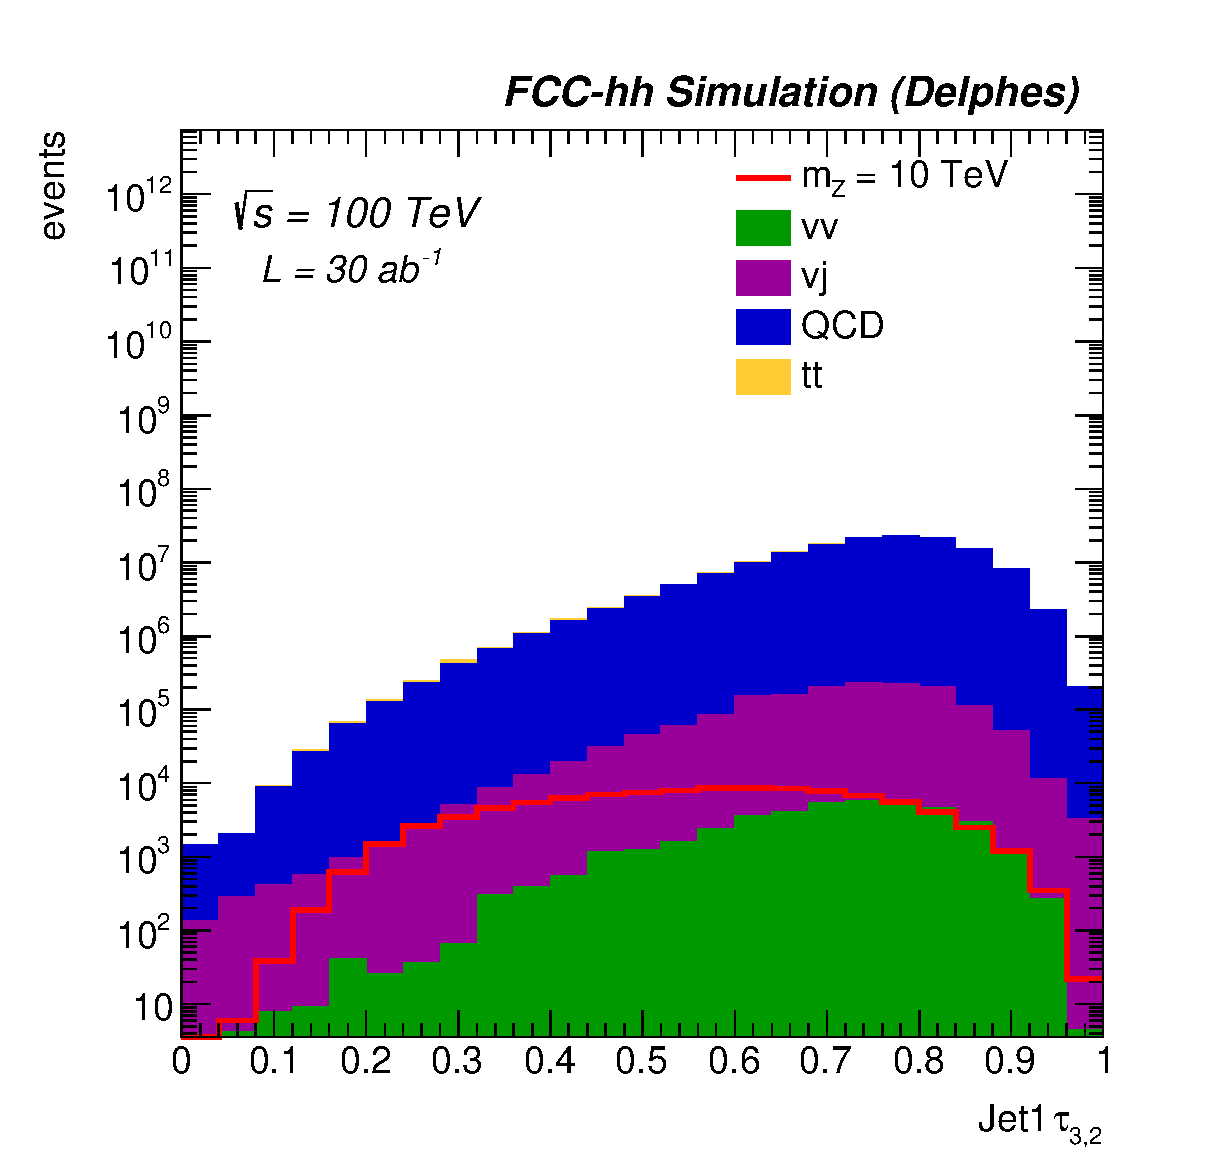
\includegraphics[width=0.495\textwidth]{Fig/Zptt/Jet1_tau32_sel0_nostack_log.eps}
\caption{Variables used for the first step of cuts in cut-based analysis at preselection level for leading jet $\pT$ in $\Zp \rightarrow \ttbar$ analysis : jet mass SD (Soft-Dropped) corrected, jet $\tau_{21}$ and jet $\tau_{32}$. The generated mass of the signal sample is 10 $\TeV$.}
\label{fig:Zptt_sel0_cut}
\end{figure}

\begin{figure}[!htb]\centering
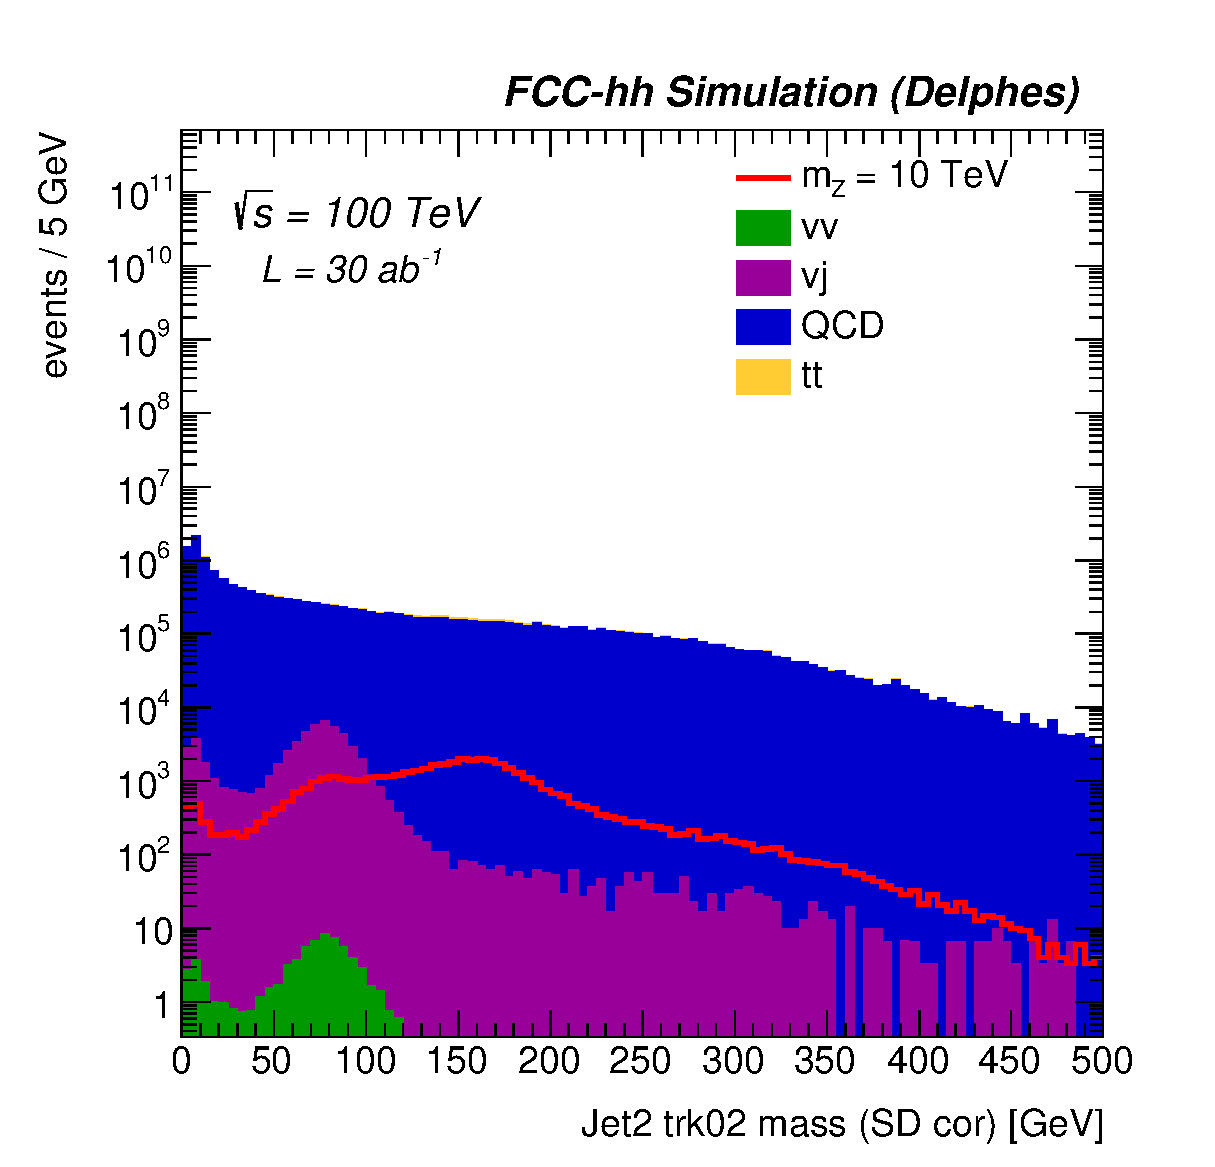
\includegraphics[width=0.495\textwidth]{Fig/Zptt/Jet2_trk02_SD_Cor_m_sel1_nostack_log.eps}
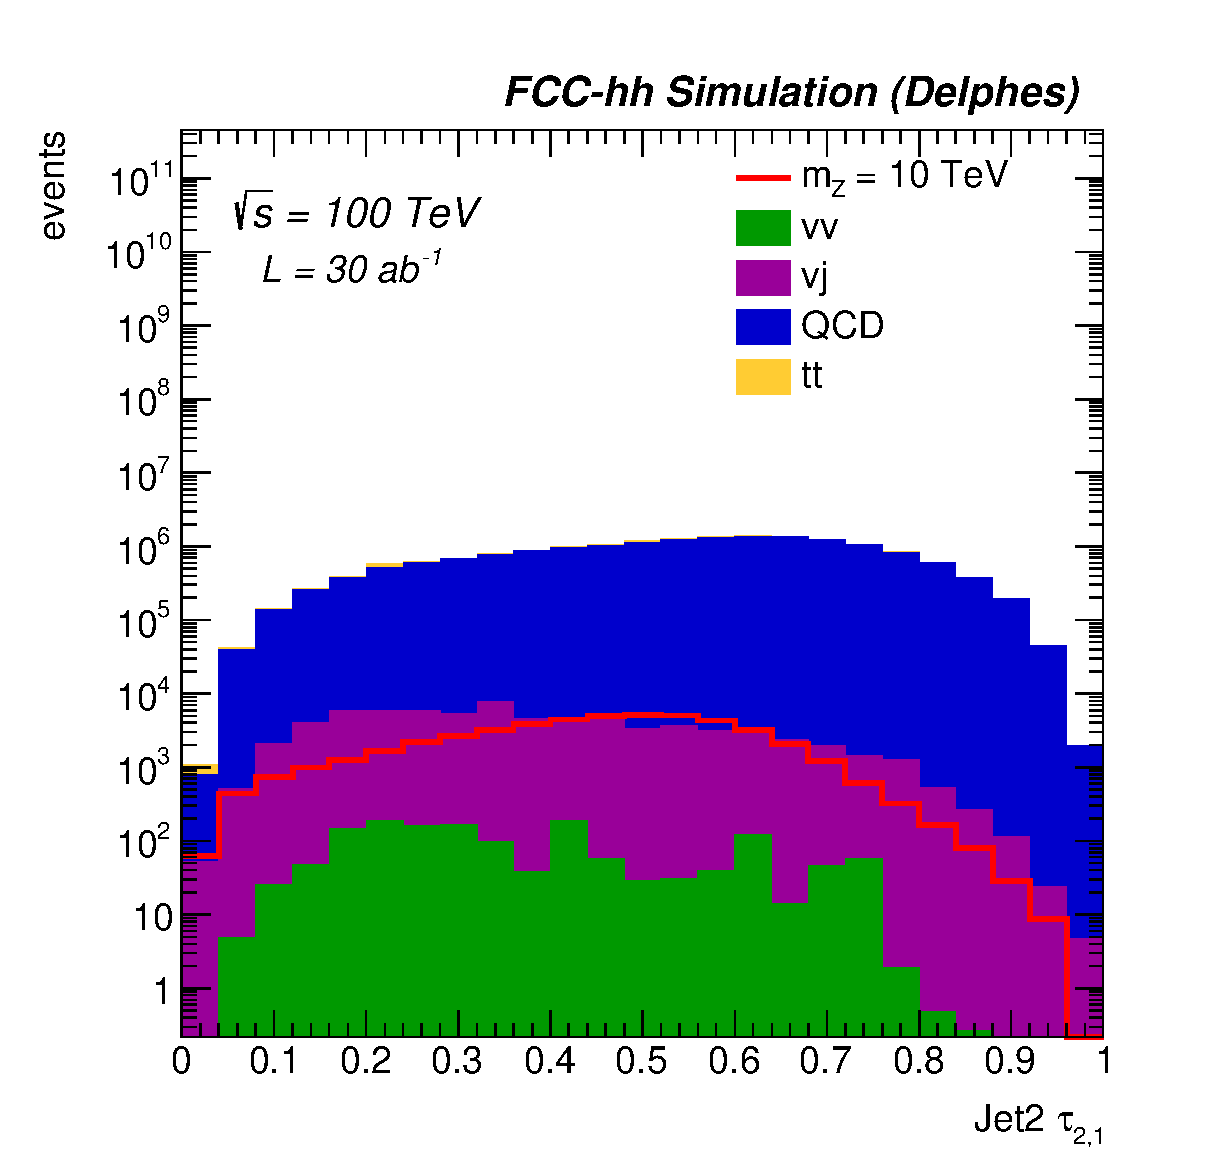
\includegraphics[width=0.495\textwidth]{Fig/Zptt/Jet2_tau21_sel1_nostack_log.eps}
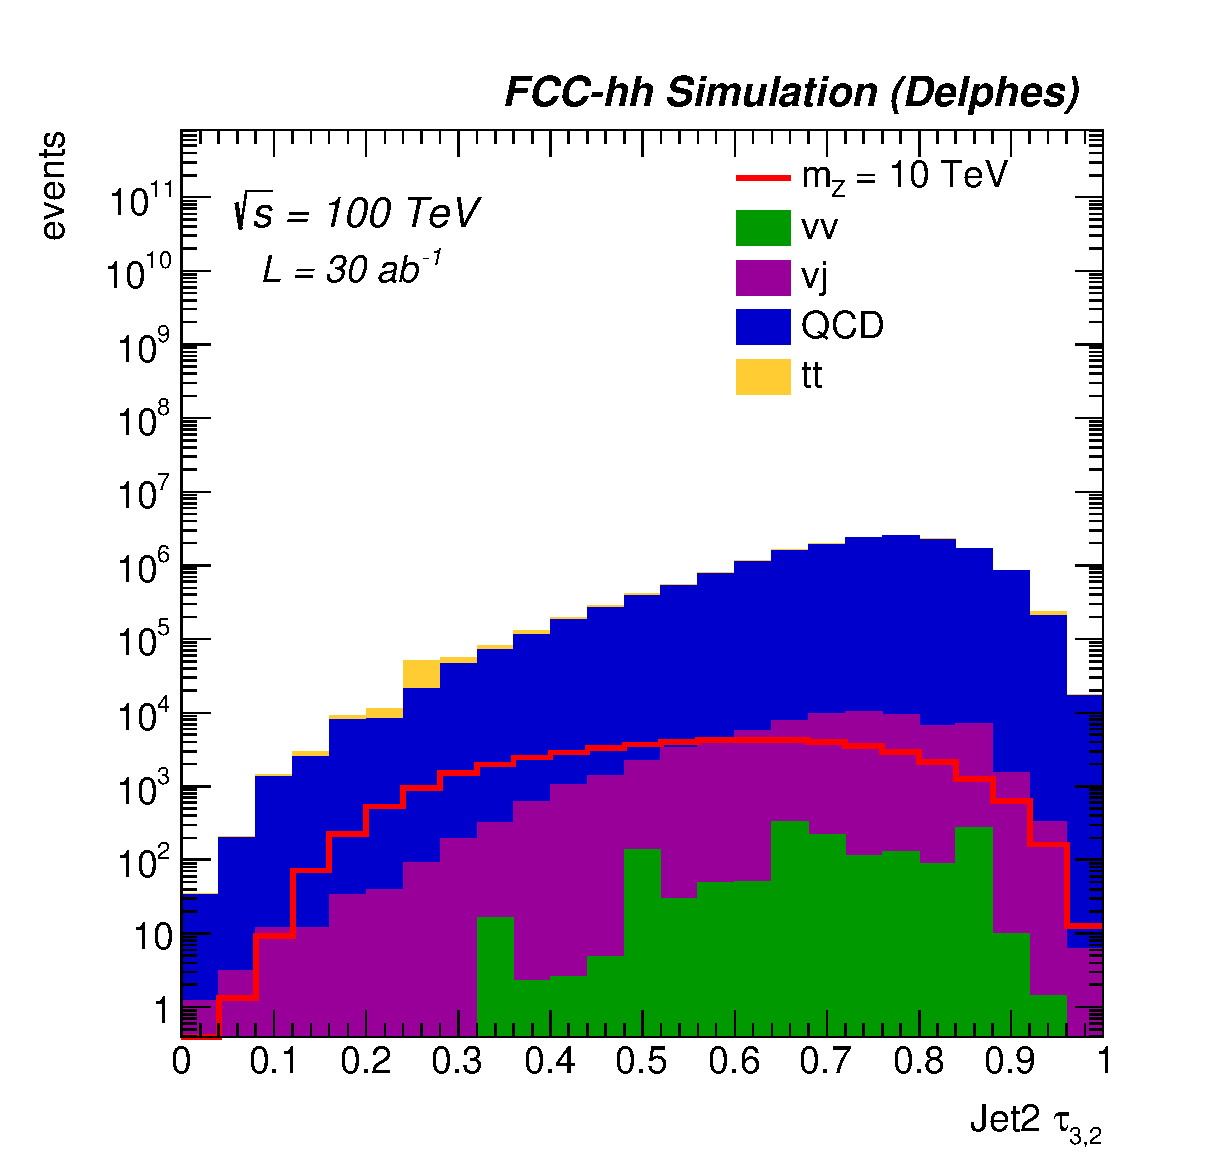
\includegraphics[width=0.495\textwidth]{Fig/Zptt/Jet2_tau32_sel1_nostack_log.eps}
\caption{Variables used for the second step of cuts in cut-based analysis after first set of cuts for second leading jet $\pT$ in $\Zp \rightarrow \ttbar$ analysis : jet mass SD (Soft-Dropped) corrected, jet $\tau_{21}$ and jet $\tau_{32}$. The generated mass of the signal sample is 10 $\TeV$.}
\label{fig:Zptt_sel1_cut}
\end{figure}

\begin{figure}[!htb]\centering
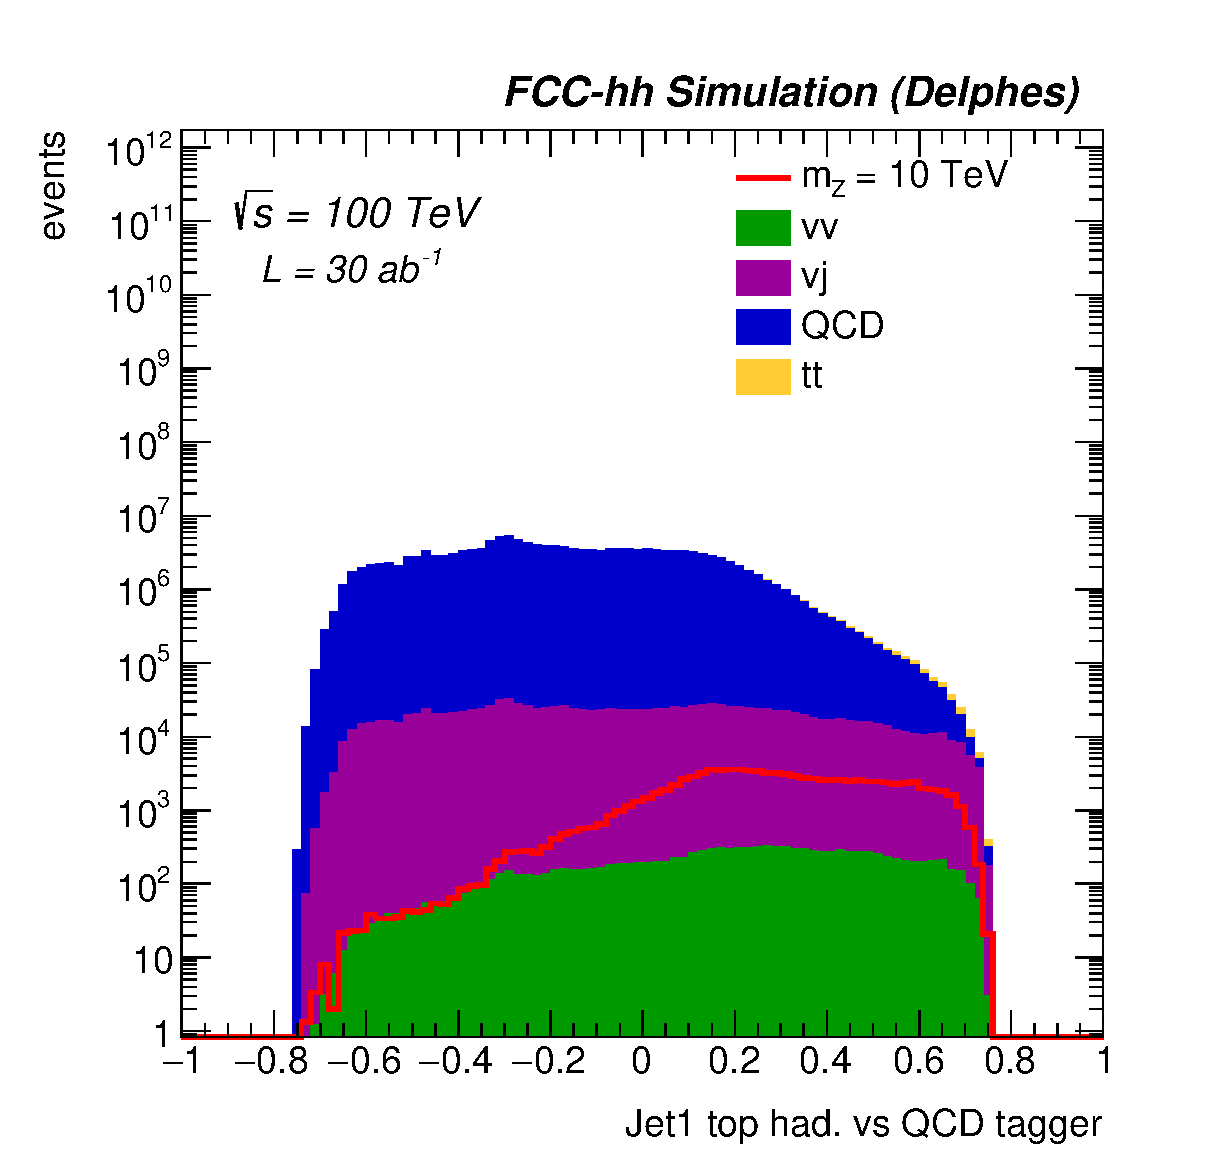
\includegraphics[width=0.495\textwidth]{Fig/Zptt/Jet1_thad_vs_QCD_tagger_sel0_nostack_log.eps}
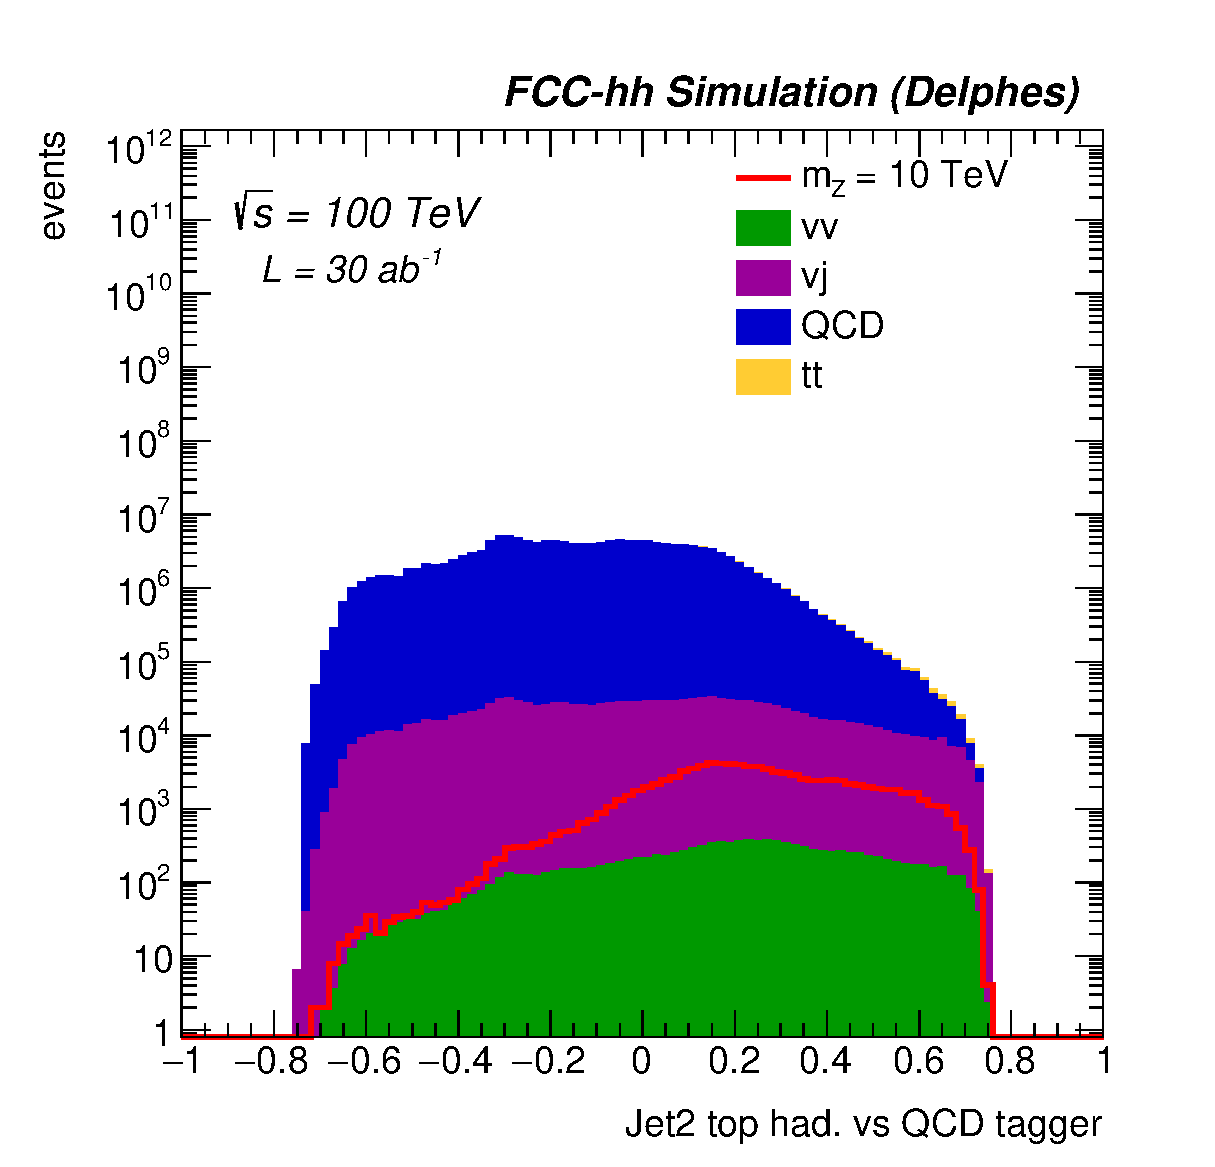
\includegraphics[width=0.495\textwidth]{Fig/Zptt/Jet2_thad_vs_QCD_tagger_sel0_nostack_log.eps}
\caption{top Vs QCD tagger at preselection level for leading jet (left) and second leading jet $\pT$ (right) in $\Zp \rightarrow \ttbar$ analysis. The generated mass of the signal sample is 10 $\TeV$.}
\label{fig:Zptt_sel0_tagger}
\end{figure}

\begin{figure}[!htb]\centering
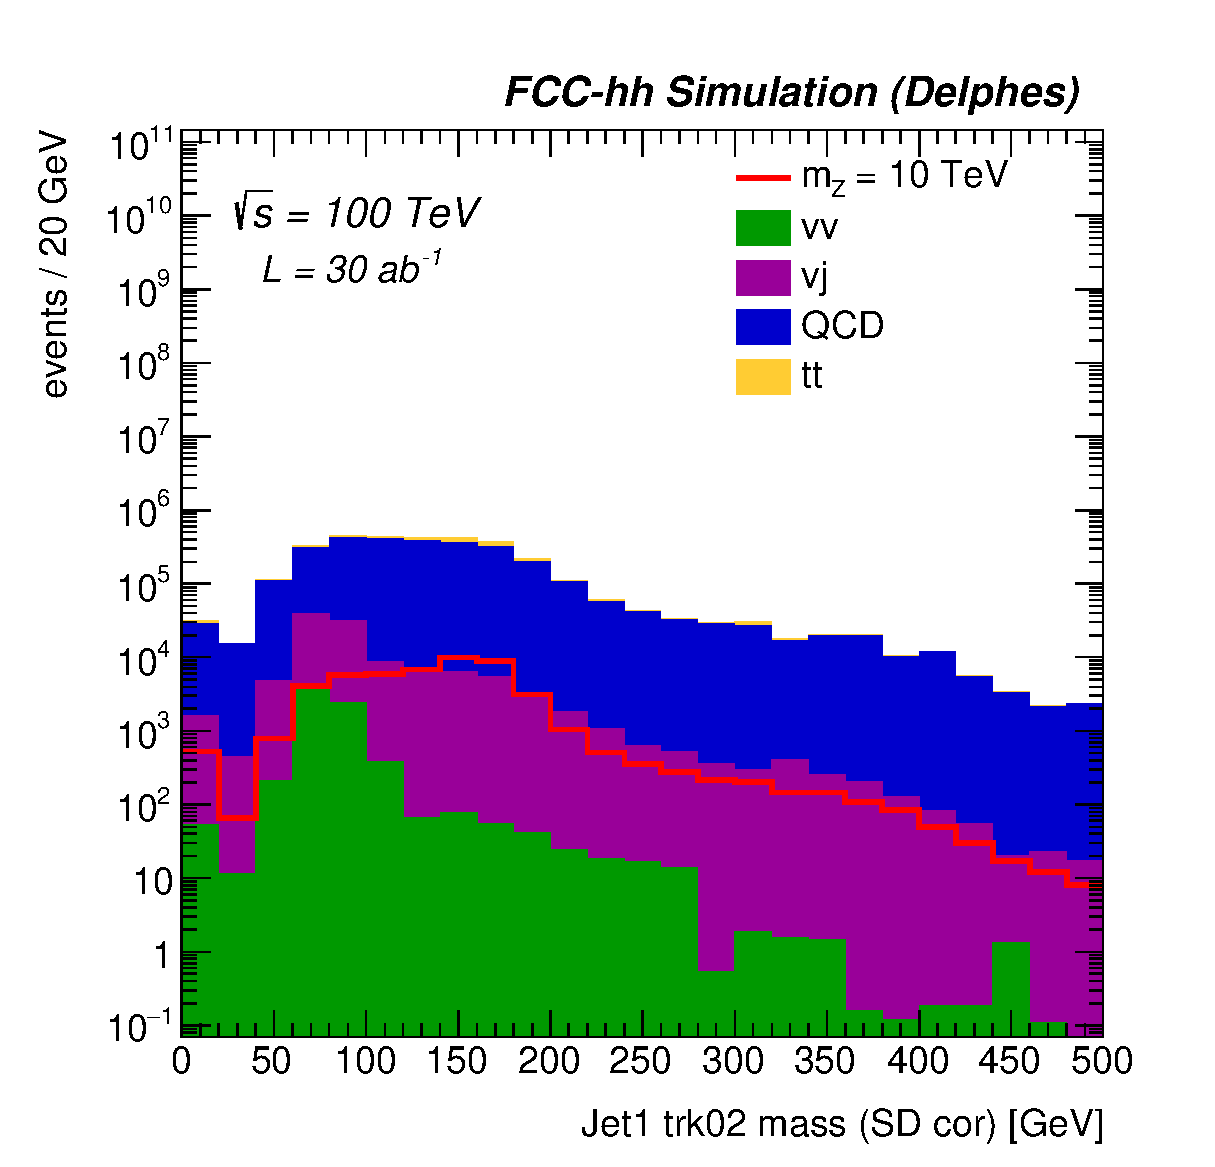
\includegraphics[width=0.495\textwidth]{Fig/Zptt/Jet1_trk02_SD_Cor_m_sel3_nostack_log.eps}
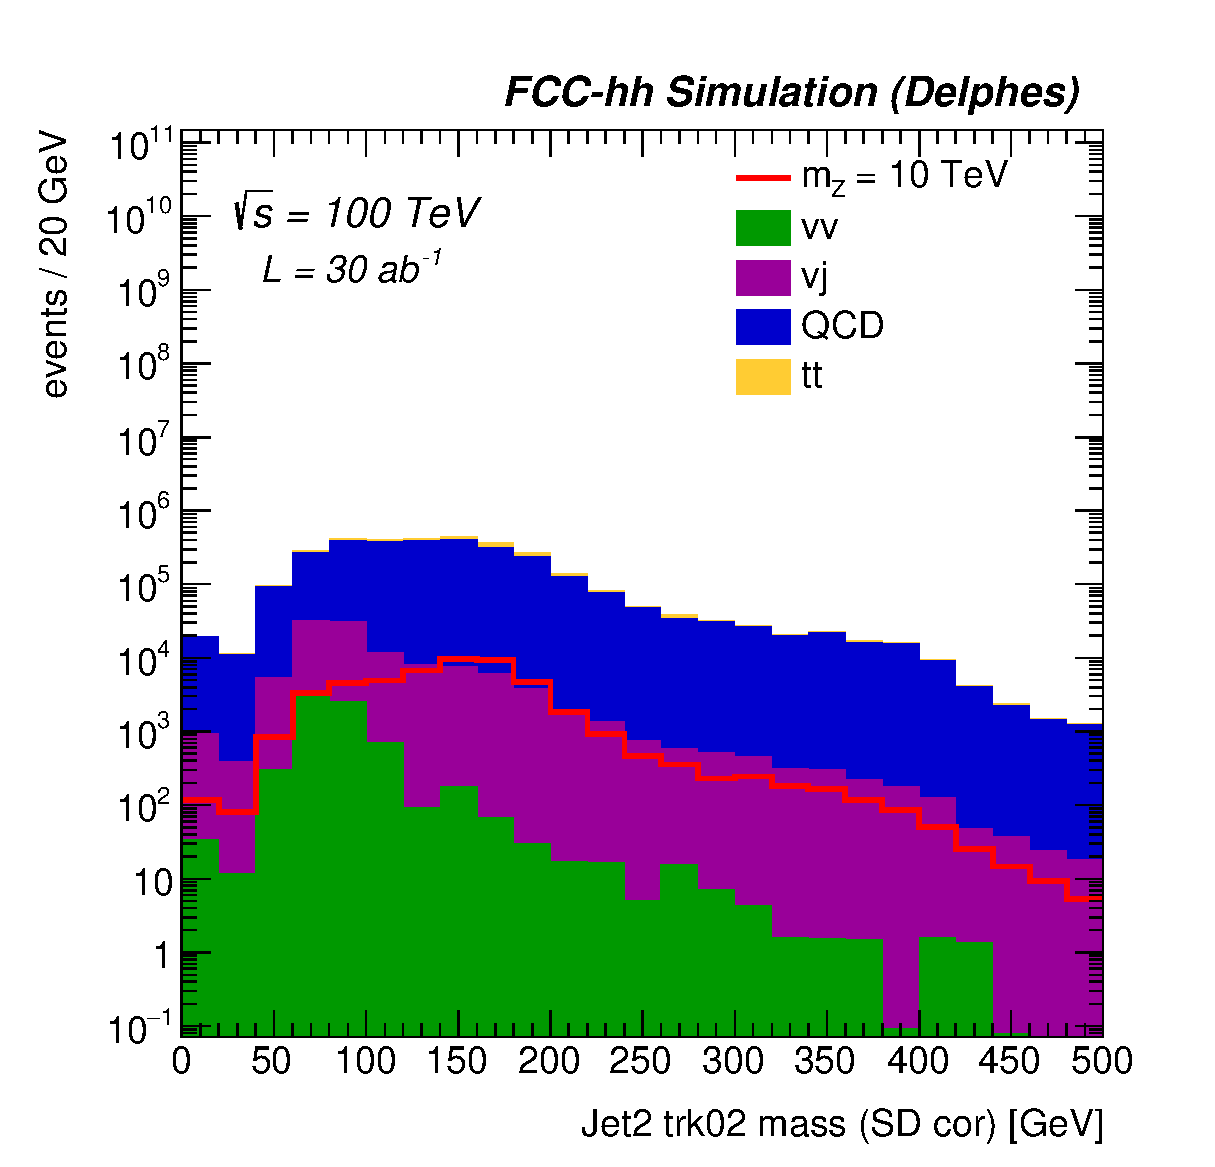
\includegraphics[width=0.495\textwidth]{Fig/Zptt/Jet2_trk02_SD_Cor_m_sel3_nostack_log.eps}
\caption{Jet mass SD (Soft-Dropped) corrected in anti-QCD tagger-based analysis after first set of cuts for leading jet (left) and second leading jet $\pT$ (right) in $\Zp \rightarrow \ttbar$ analysis. The generated mass of the signal sample is 10 $\TeV$.}
\label{fig:RSGww_sel1_tagger}
\end{figure}

% no eps
\begin{figure}[!htb]\centering
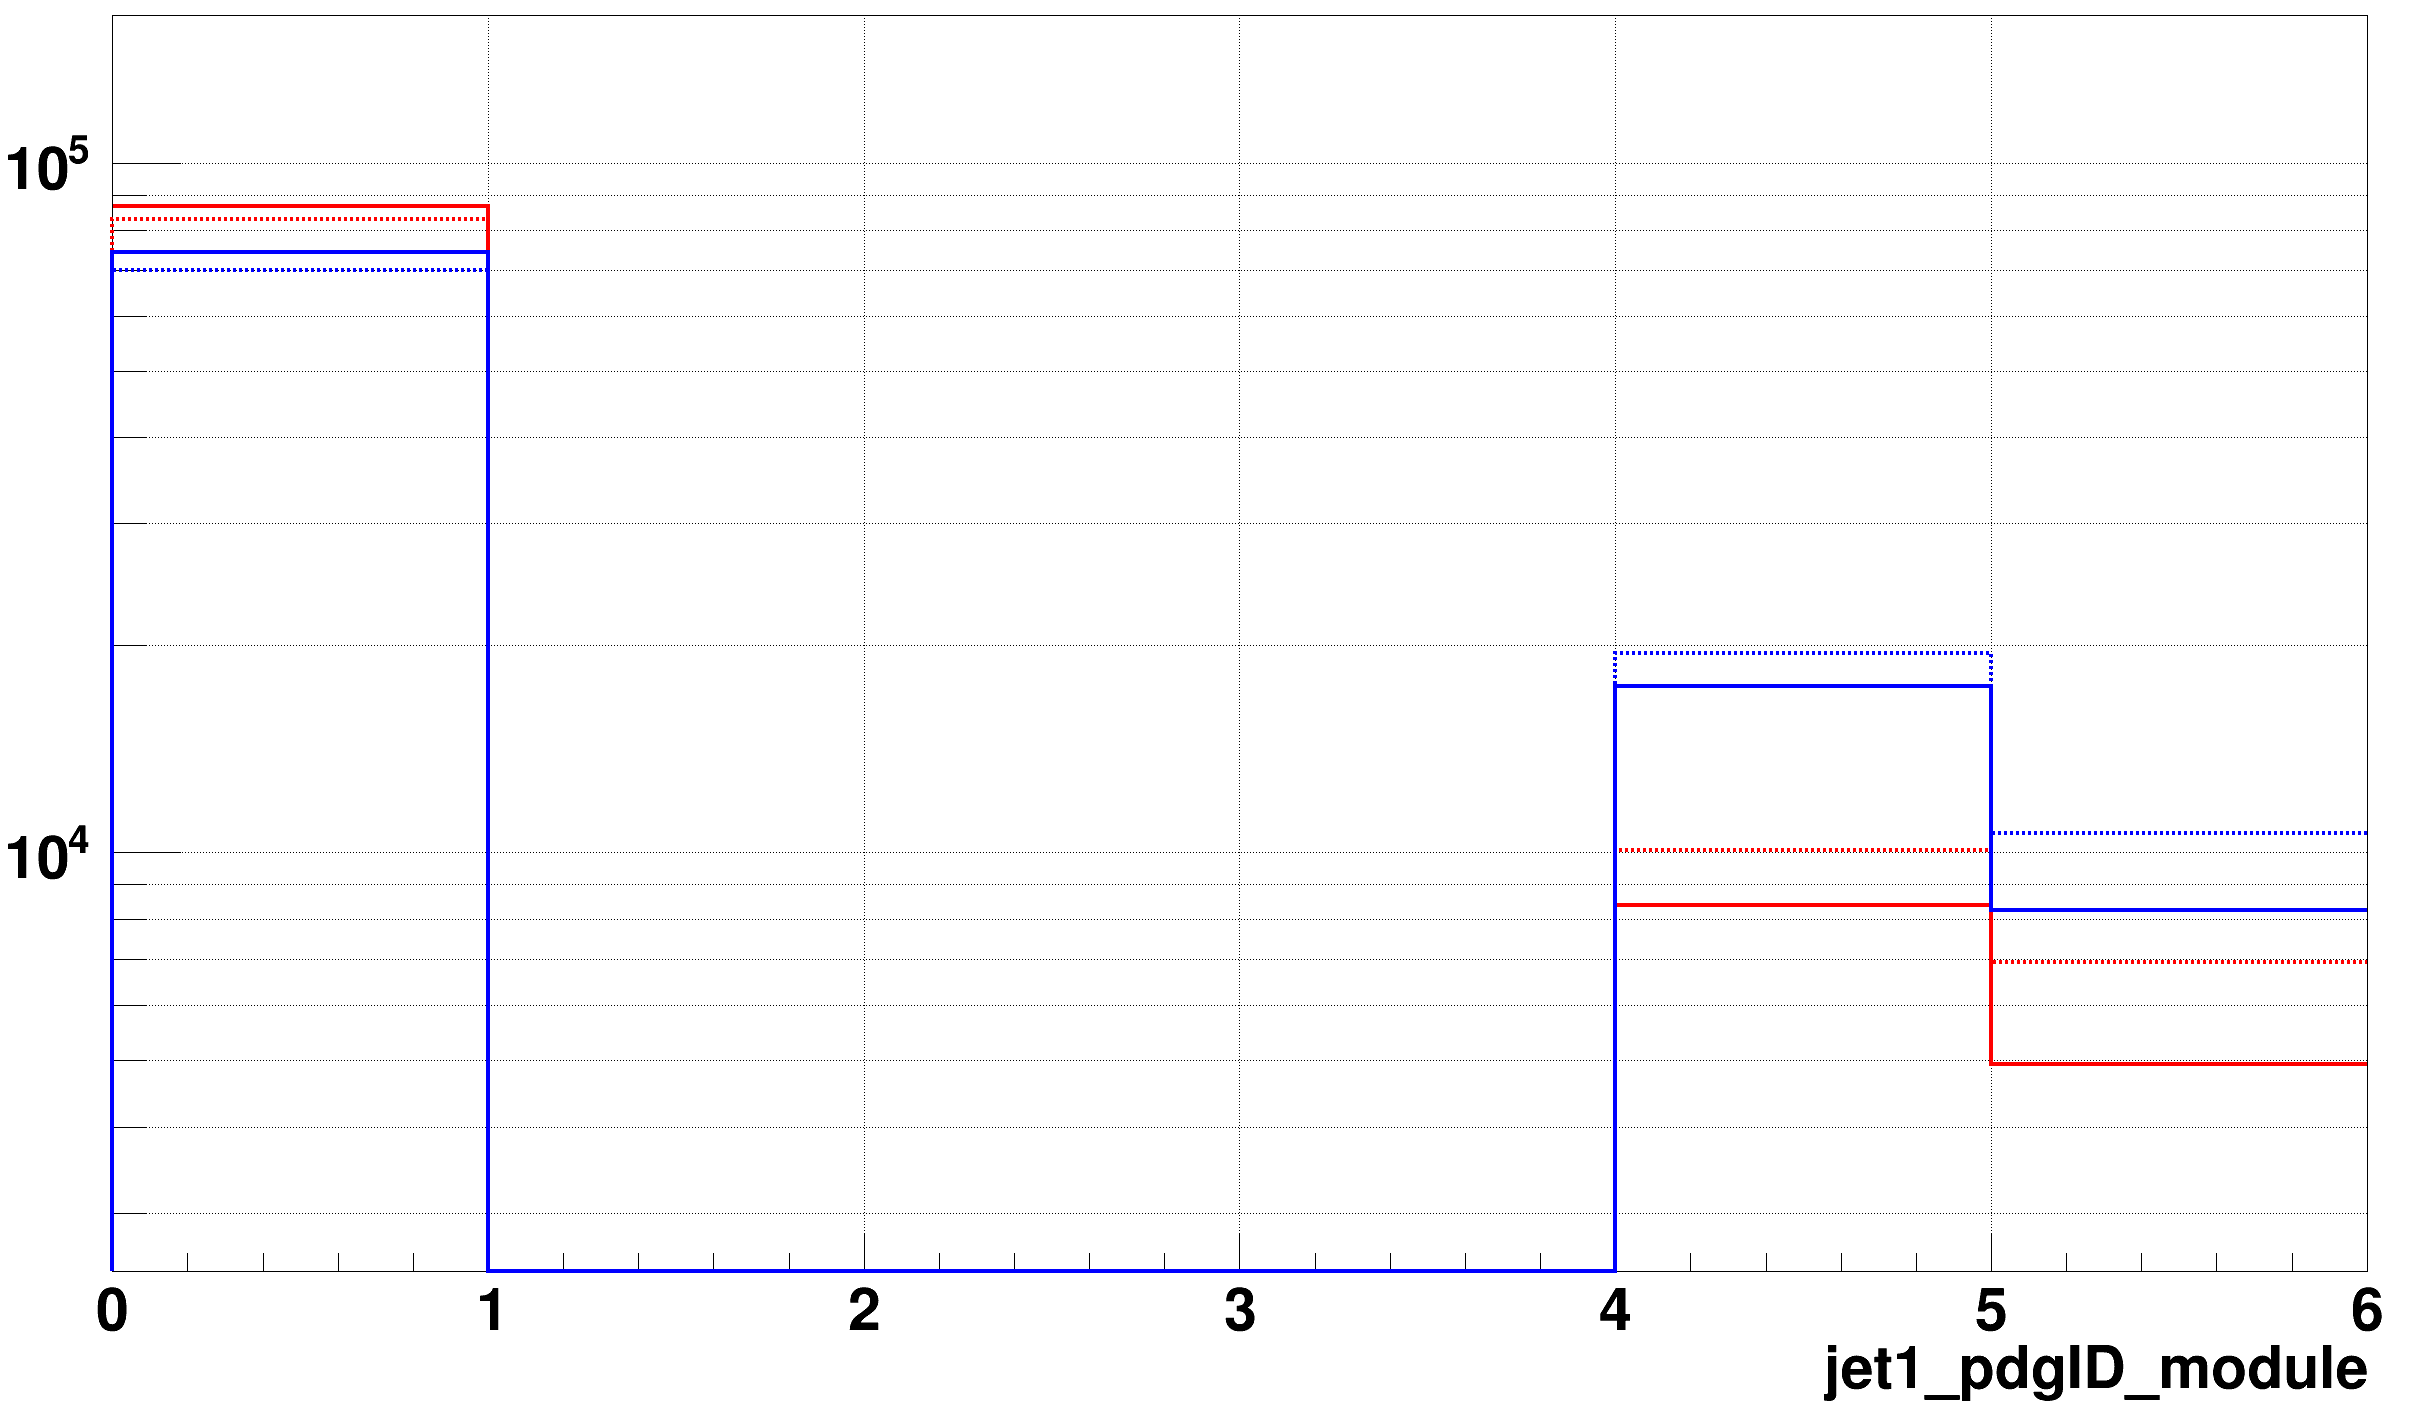
\includegraphics[width=0.495\textwidth]{Fig/check_TRF/Zptt/jet12pdgID_QCD5f_redModule_blueDELPHES.png}
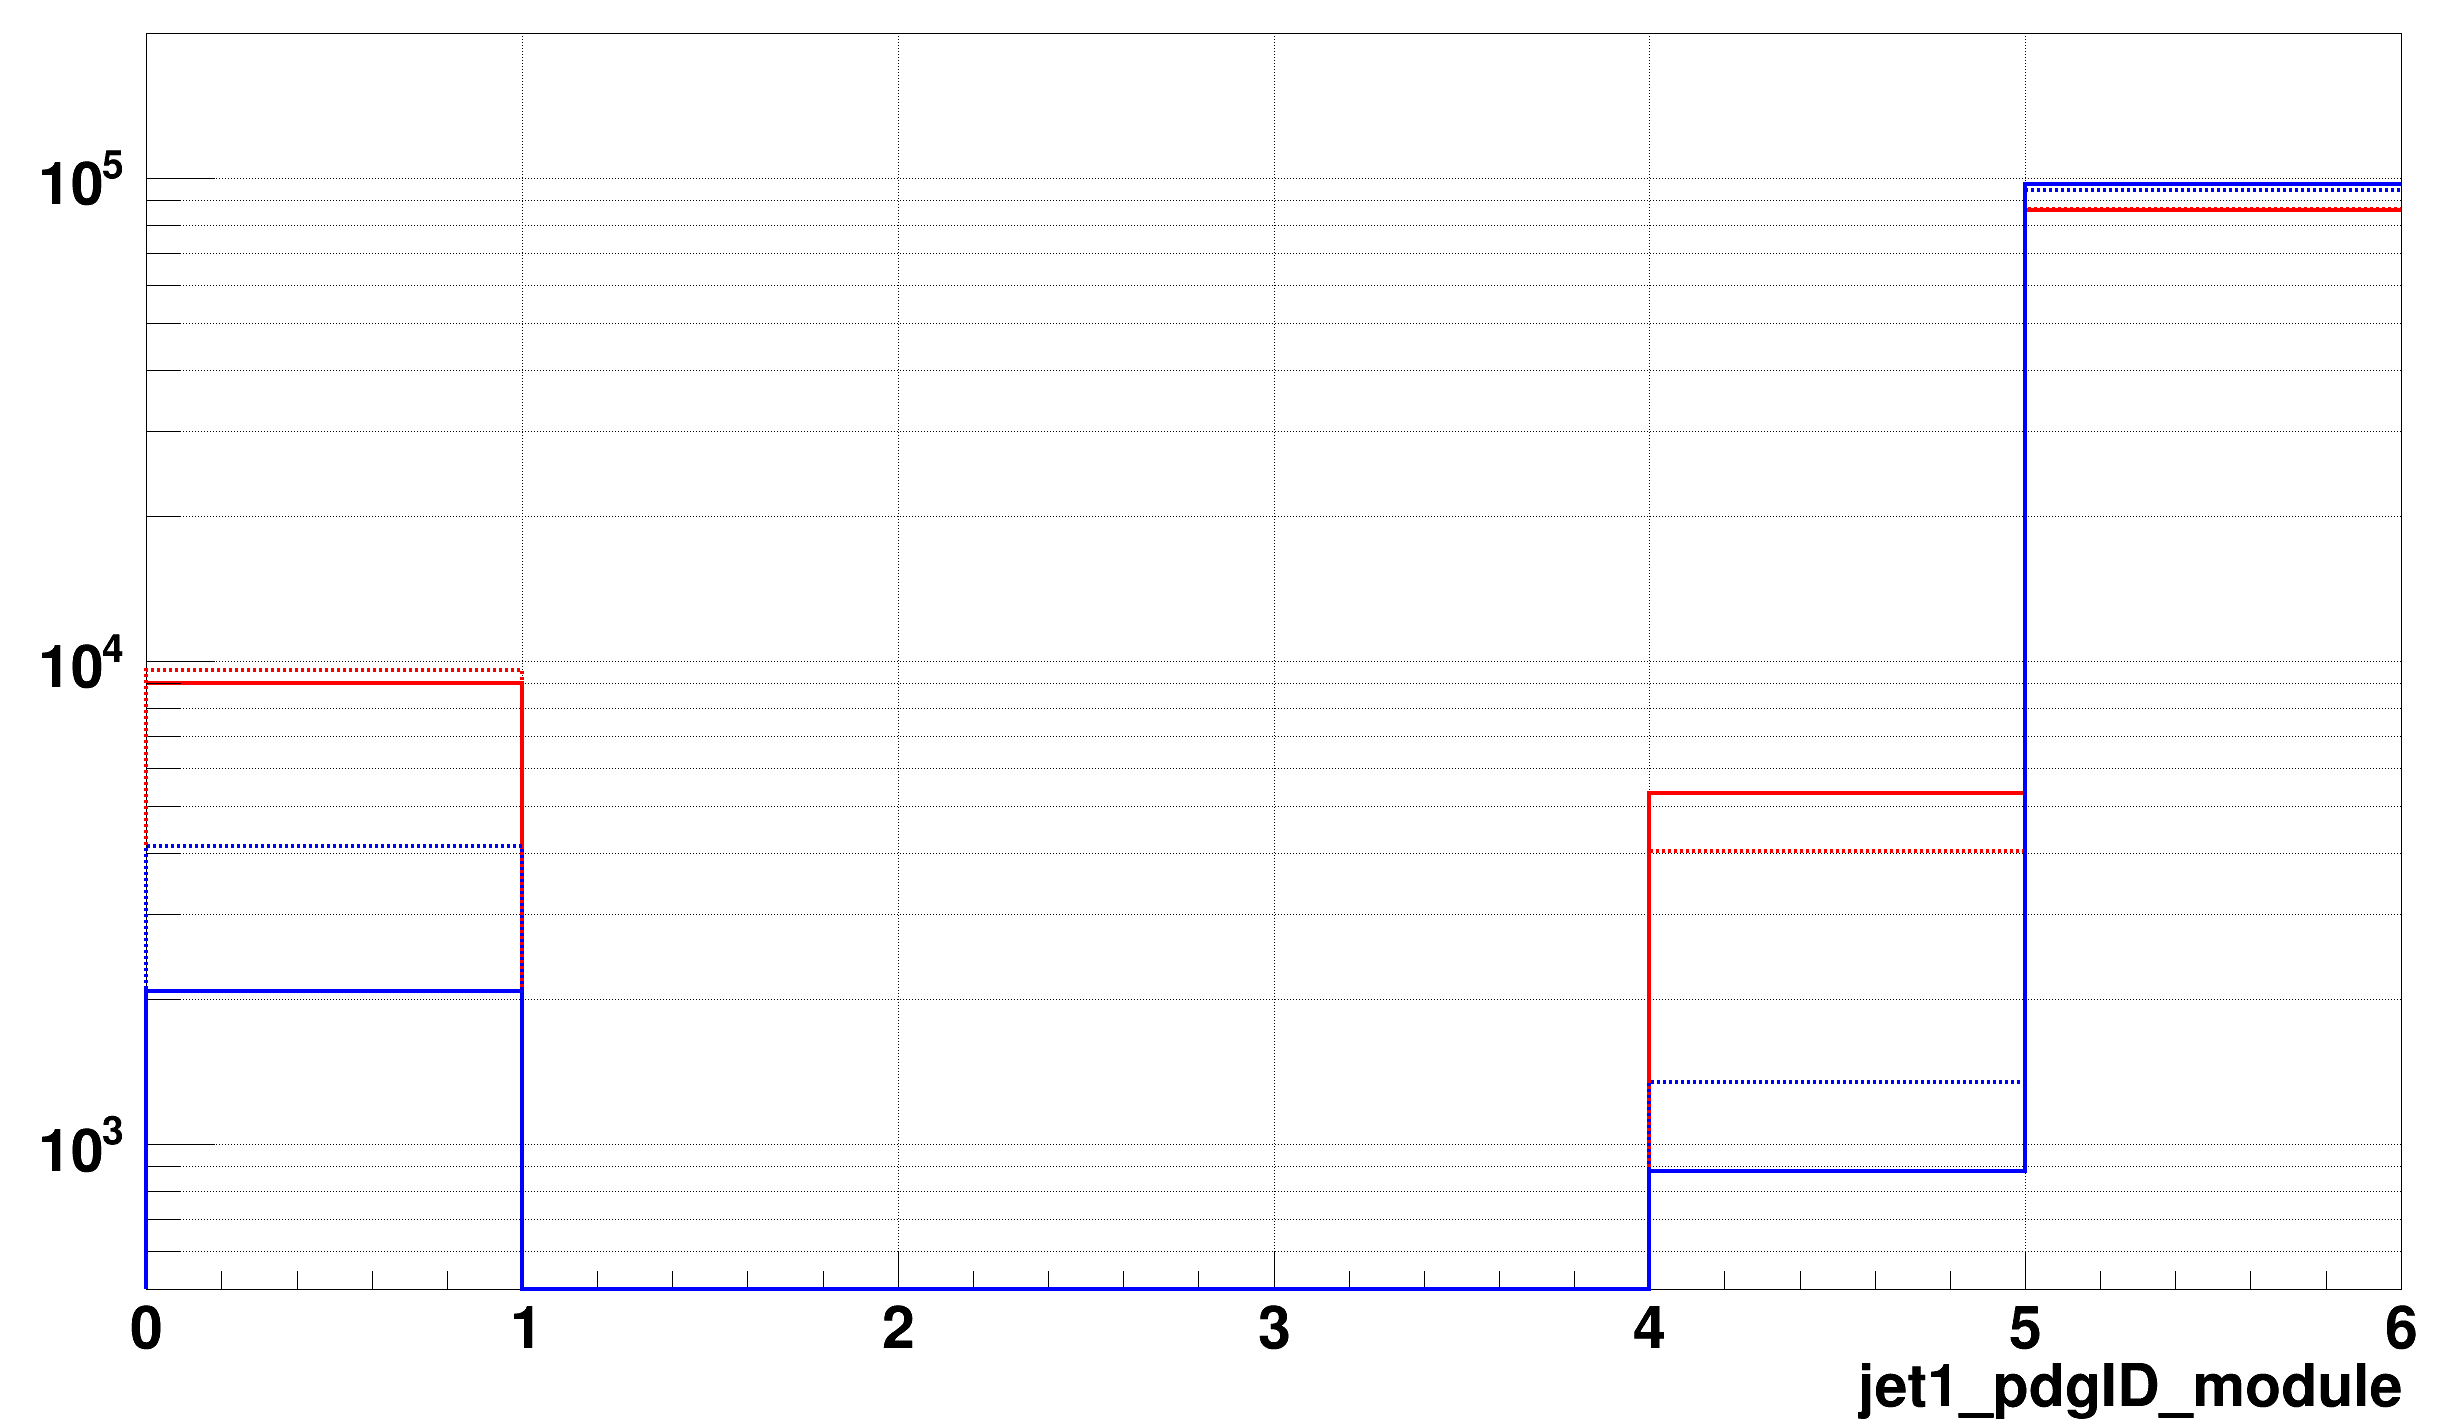
\includegraphics[width=0.495\textwidth]{Fig/check_TRF/Zptt/jet12pdgID_ttbar_redModule_blueDELPHES.png}
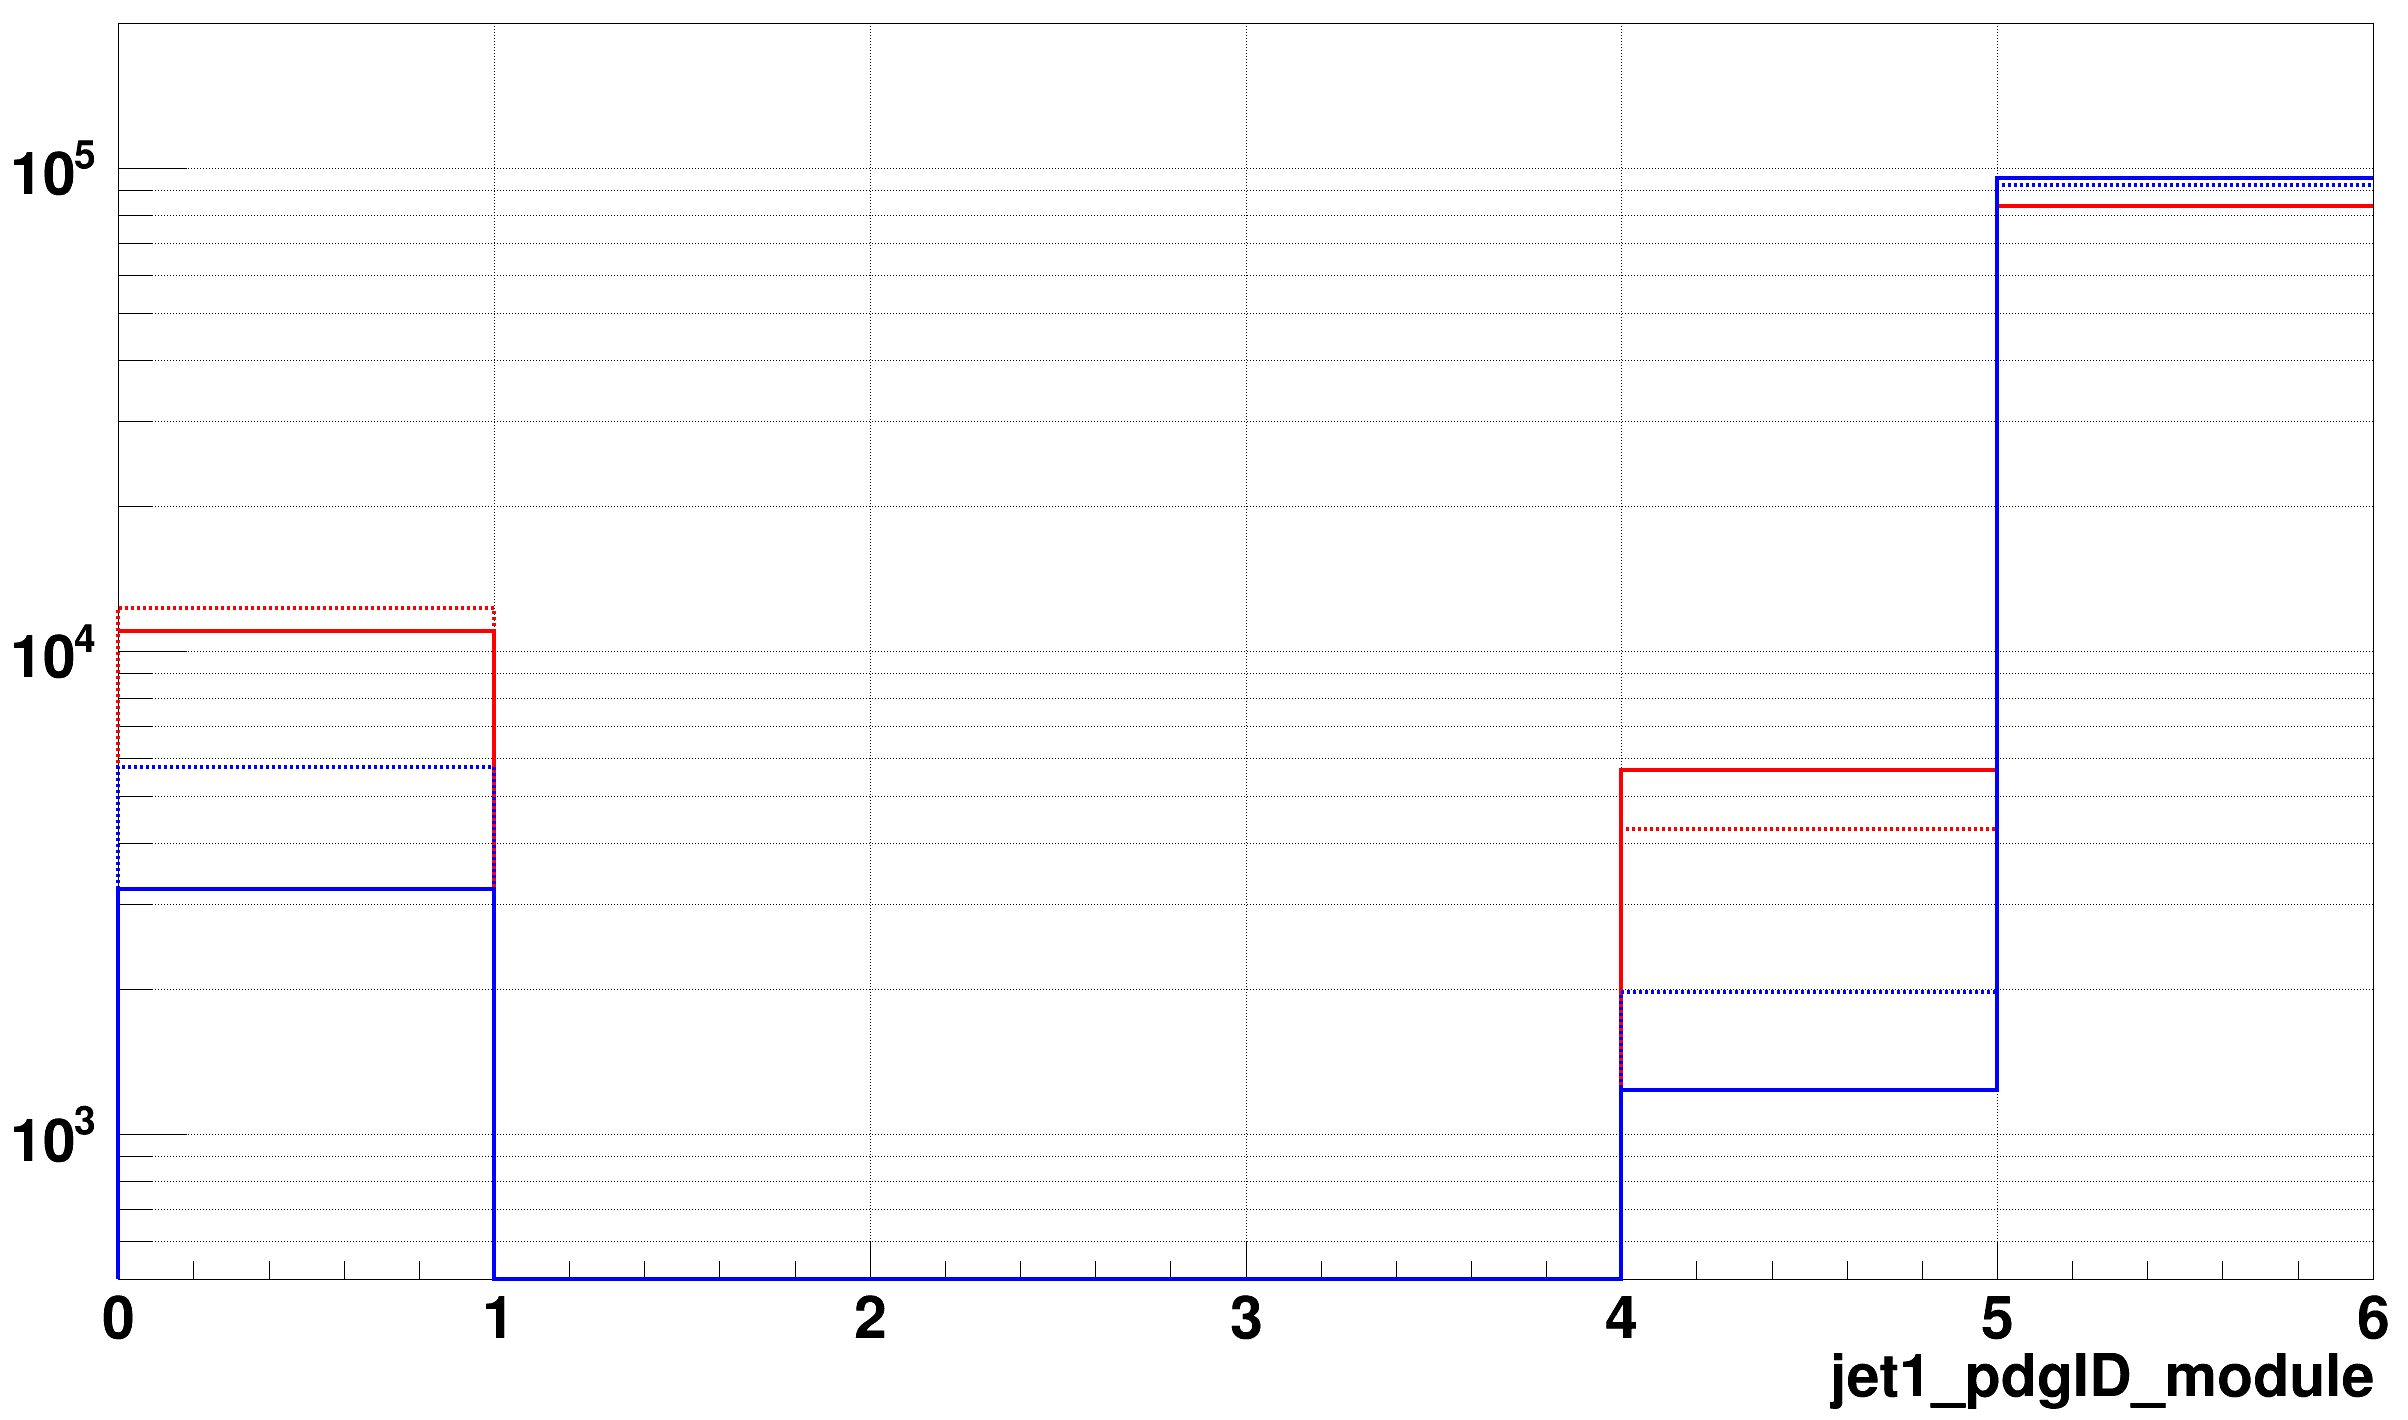
\includegraphics[width=0.495\textwidth]{Fig/check_TRF/Zptt/jet12pdgID_Zptt10TeV_redModule_blueDELPHES.png}
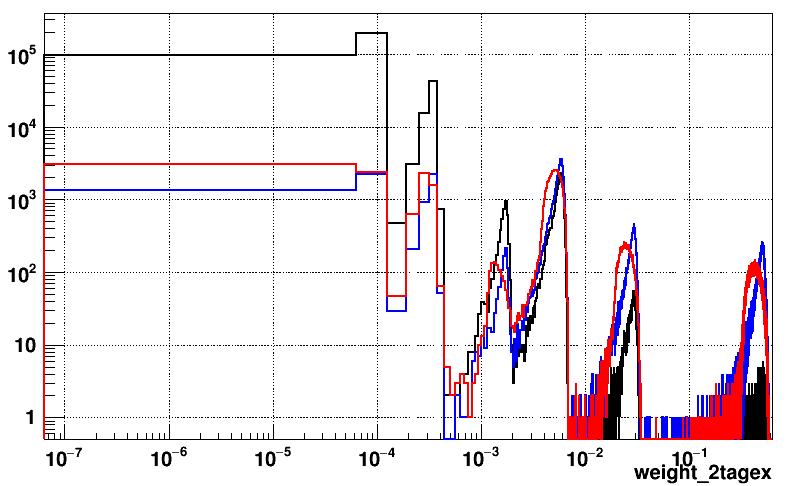
\includegraphics[width=0.495\textwidth]{Fig/check_TRF/Zptt/TRF2tagex_module_redZptt10TeV_blackQCD_bluettbar.png}
\caption{Checks of pdgID obtained from recomputation (red) compared to Delphes information (blue) for leading jet (continuous line) and second leading jet $\pT$ (dashed line), and for QCD (top left), $\ttbar$ (top right) and $\Zp \rightarrow \ttbar$ 10 $\TeV$ (bottom left) samples in $\Zp \rightarrow \ttbar$ analysis. Tag Rate Function for a two b-tagged jets event computed from the two leading jets only of the event (bottom right) for QCD (black), $\ttbar$ blue) and $\Zp \rightarrow \ttbar$ 10 $\TeV$ (red) samples.}
\label{fig:Zptt_TRFchecks}
\end{figure}

% no eps
\begin{figure}[!htb]\centering
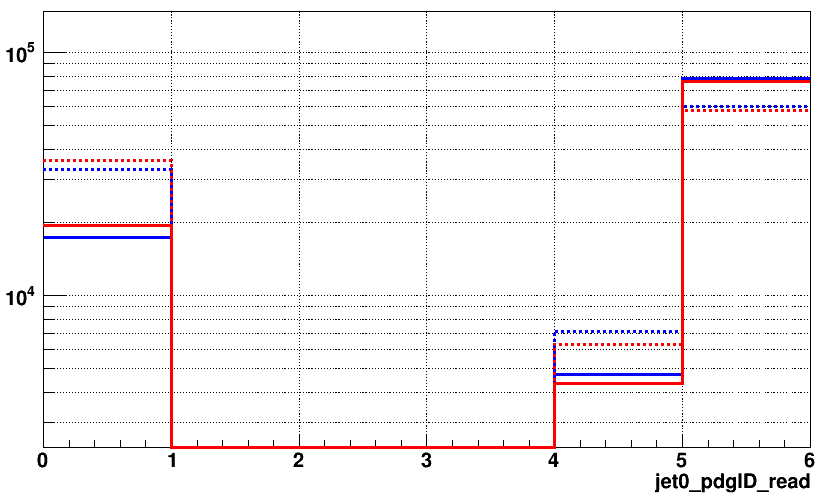
\includegraphics[width=0.495\textwidth]{Fig/check_TRF/tth_boosted/jet12pdgID_ttbb_redModule_blueDELPHES.png}
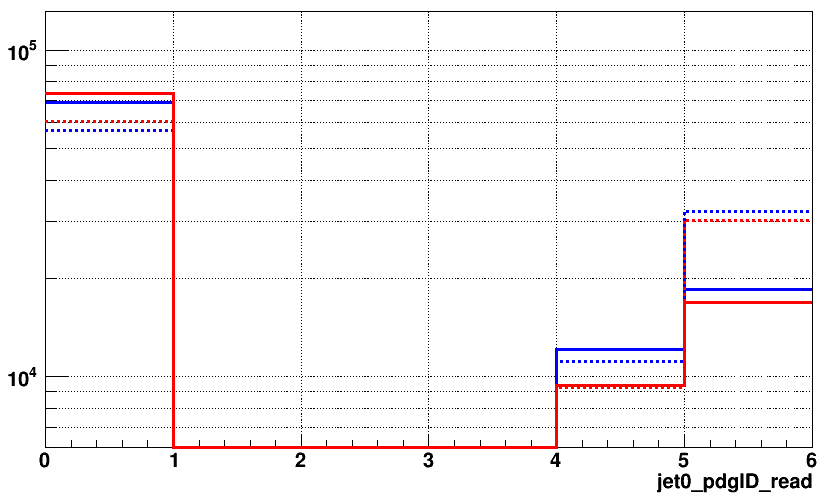
\includegraphics[width=0.495\textwidth]{Fig/check_TRF/tth_boosted/jet12pdgID_ttj_redModule_blueDELPHES.png}
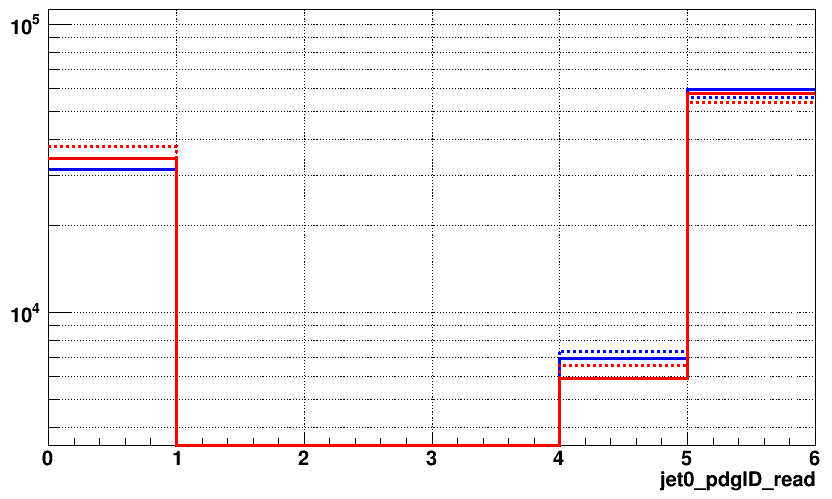
\includegraphics[width=0.495\textwidth]{Fig/check_TRF/tth_boosted/jet12pdgID_ttz_redModule_blueDELPHES.png}
\includegraphics[width=0.495\textwidth]{Fig/check_TRF/tth_boosted/jet12pdgID_tth_redModule_blueDELPHES.png}
\caption{Checks of pdgID obtained from recomputation (red) compared to Delphes information (blue) for leading jet (continuous line) and second leading jet $\pT$ (dashed line), and for $\ttbb$ (top left), $\ttj$ (top right), $\ttz$ (bottom left) and $\tthbb$ (bottom right) samples in $\tthbb$ boosted analysis.}
\label{fig:tthboosted_TRFchecks1}
\end{figure}

% no eps
\begin{figure}[!htb]\centering
\includegraphics[width=0.495\textwidth]{Fig/check_TRF/tth_boosted/jet34pdgID_ttbb_redModule_blueDELPHES.png}
\includegraphics[width=0.495\textwidth]{Fig/check_TRF/tth_boosted/jet34pdgID_ttj_redModule_blueDELPHES.png}
\includegraphics[width=0.495\textwidth]{Fig/check_TRF/tth_boosted/jet34pdgID_ttz_redModule_blueDELPHES.png}
\includegraphics[width=0.495\textwidth]{Fig/check_TRF/tth_boosted/jet34pdgID_tth_redModule_blueDELPHES.png}
\caption{Checks of pdgID obtained from recomputation (red) compared to Delphes information (blue) for third leading jet (continuous line) and fourth leading jet $\pT$ (dashed line), and for $\ttbb$ (top left), $\ttj$ (top right), $\ttz$ (bottom left) and $\tthbb$ (bottom right) samples in $\tthbb$ boosted analysis.}
\label{fig:tthboosted_TRFchecks2}
\end{figure}

\begin{figure}[!htb]\centering
\includegraphics[width=0.495\textwidth]{Fig/Zptt/Mj1j2_pf08_MetCorr_sel2_nostack_log.eps}
\includegraphics[width=0.495\textwidth]{Fig/Zptt/Mj1j2_pf08_MetCorr_sel4_nostack_log.eps}
\includegraphics[width=0.495\textwidth]{Fig/Zptt/Mj1j2_pf08_MetCorr_sel5_nostack_log.eps}
\includegraphics[width=0.495\textwidth]{Fig/Zptt/Mj1j2_pf08_MetCorr_sel6_nostack_log.eps}
\includegraphics[width=0.495\textwidth]{Fig/Zptt/Mj1j2_pf08_MetCorr_sel7_nostack_log.eps}
\includegraphics[width=0.495\textwidth]{Fig/Zptt/Mj1j2_pf08_MetCorr_sel8_nostack_log.eps}
\caption{Zprime mass after the full selection for anaylsis cut-based (left) and anti-QCD tagger based (right), and for the b-tagging scenarios : before b-tag (top), direct 2 b-tag (middle) and Tag Rate Function 2 b-tag (bottom) in $\Zp \rightarrow \ttbar$ analysis. The generated mass of the signal sample is 10 $\TeV$.}
\label{fig:Zptt_mass_sel_final}
\end{figure}

\begin{figure}[!htb]\centering
\includegraphics[width=0.495\textwidth]{Fig/Zptt/lim_Zprime_tt_fcc_v02_cut.eps}
\includegraphics[width=0.495\textwidth]{Fig/Zptt/DiscoveryPotential_tt_cut_rootStyle.eps}
\includegraphics[width=0.495\textwidth]{Fig/Zptt/lim_Zprime_tt_fcc_v02_tagger.eps}
\includegraphics[width=0.495\textwidth]{Fig/Zptt/DiscoveryPotential_tt_TC2_tagger_rootStyle.eps}
\caption{Limit (left) and discovery potential (right) for analysis cut-based with direct b-tagging (top) and anti-QCD tagger-based with direct b-tagging (bottom) in $\Zp \rightarrow \ttbar$ analysis. Default model used for discovery potential is TC2.}
\label{fig:Zptt_limit_direct}
\end{figure}

\begin{figure}[!htb]\centering
\includegraphics[width=0.495\textwidth]{Fig/Zptt/lim_Zprime_tt_fcc_v02_cut_TRFbtag.eps}
\includegraphics[width=0.495\textwidth]{Fig/Zptt/DiscoveryPotential_tt_cut_TRFbtag_rootStyle.eps}
\includegraphics[width=0.495\textwidth]{Fig/Zptt/lim_Zprime_tt_fcc_v02_tagger_TRFbtag.eps}
\includegraphics[width=0.495\textwidth]{Fig/Zptt/DiscoveryPotential_tt_SSM_TC2_tagger_TRFbtag_rootStyle.eps}
\caption{Limit (left) and discovery potential (right) for analysis cut-based with TRF b-tagging (top) and anti-QCD tagger-based with TRF b-tagging (bottom) in $\Zp \rightarrow \ttbar$ analysis. Default model used for discovery potential is TC2 in the top plot. The bottom discovery plot shows the comparison between the TC2 default model (red line) and the SSM one (blue line).}
\label{fig:Zptt_limit_trf}
\end{figure}


\subsection{$G \rightarrow WW$}
\label{subsec:RSGww}

Backgrounds: QCD multijet, V+jets, VV.

\begin{figure}[!htb]\centering
\includegraphics[width=0.8\textwidth]{Fig/RSGww/rapiditySeparation_sel0_before_cut_nostack_log.eps}
\caption{Rapidity separation at preselection level before cut on this variable in $G \rightarrow WW$ analysis. The generated mass of the signal sample is 10 $\TeV$.}
\label{fig:RSGww_sel0_rapidity}
\end{figure}

\begin{figure}[!htb]\centering
\includegraphics[width=0.495\textwidth]{Fig/RSGww/Jet1_trk02_SD_Cor_m_sel0_nostack_log.eps}
\includegraphics[width=0.495\textwidth]{Fig/RSGww/Jet2_trk02_SD_Cor_m_sel0_nostack_log.eps}
\includegraphics[width=0.495\textwidth]{Fig/RSGww/Jet1_tau21_sel0_nostack_log.eps}
\includegraphics[width=0.495\textwidth]{Fig/RSGww/Jet2_tau21_sel0_nostack_log.eps}
\caption{Variables used for the first step of cuts in cut-based analysis at preselection level for leading jet (left) and second leading jet $\pT$ (right) in $G \rightarrow WW$ analysis : jet mass SD (Soft-Dropped) corrected (top) and jet $\tau_{21}$ (bottom). The generated mass of the signal sample is 10 $\TeV$.}
\label{fig:RSGww_sel0_cut}
\end{figure}

\begin{figure}[!htb]\centering
\includegraphics[width=0.495\textwidth]{Fig/RSGww/Jet1_Flow45_sel1_nostack_log.eps}
\includegraphics[width=0.495\textwidth]{Fig/RSGww/Jet2_Flow45_sel1_nostack_log.eps}
\includegraphics[width=0.495\textwidth]{Fig/RSGww/Jet1_Flow55_sel1_nostack_log.eps}
\includegraphics[width=0.495\textwidth]{Fig/RSGww/Jet2_Flow55_sel1_nostack_log.eps}
\caption{Variables used for the second step of cuts in cut-based analysis after first set of cuts for leading jet (left) and second leading jet $\pT$ (right) in $G \rightarrow WW$ analysis : jet Flow45 (top) and Flow55 (bottom). The generated mass of the signal sample is 10 $\TeV$.}
\label{fig:RSGww_sel1_cut}
\end{figure}

\begin{figure}[!htb]\centering
\includegraphics[width=0.495\textwidth]{Fig/RSGww/Jet1_Whad_vs_QCD_tagger_sel0_nostack_log.eps}
\includegraphics[width=0.495\textwidth]{Fig/RSGww/Jet2_Whad_vs_QCD_tagger_sel0_nostack_log.eps}
\caption{W Vs QCD tagger at preselection level for leading jet (left) and second leading jet $\pT$ (right) in $G \rightarrow WW$ analysis. The generated mass of the signal sample is 10 $\TeV$.}
\label{fig:RSGww_sel0_tagger}
\end{figure}

\begin{figure}[!htb]\centering
\includegraphics[width=0.495\textwidth]{Fig/RSGww/Jet1_trk02_SD_Cor_m_sel3_nostack_log.eps}
\includegraphics[width=0.495\textwidth]{Fig/RSGww/Jet2_trk02_SD_Cor_m_sel3_nostack_log.eps}
\caption{Jet mass SD (Soft-Dropped) corrected in anti-QCD tagger-based analysis after first set of cuts for leading jet (left) and second leading jet $\pT$ (right) in $G \rightarrow WW$ analysis. The generated mass of the signal sample is 10 $\TeV$.}
\label{fig:RSGww_sel1_tagger}
\end{figure}

\begin{figure}[!htb]\centering
\includegraphics[width=0.495\textwidth]{Fig/RSGww/Mj1j2_pf08_sel2_nostack_log.eps}
\includegraphics[width=0.495\textwidth]{Fig/RSGww/Mj1j2_pf08_sel4_nostack_log.eps}
\caption{RSG mass after the full selection for analysis cut-based (left) and anti-QCD tagger-based (right). The generated mass of the signal sample is 10 $\TeV$.}
\label{fig:RSGww_mass_sel_final}
\end{figure}

\begin{figure}[!htb]\centering
\includegraphics[width=0.495\textwidth]{Fig/RSGww/lim_RSGraviton_ww_fcc_v02_cut.eps}
\includegraphics[width=0.495\textwidth]{Fig/RSGww/DiscoveryPotential_ww_cut_rootStyle.eps}
\includegraphics[width=0.495\textwidth]{Fig/RSGww/lim_RSGraviton_ww_fcc_v02_tagger.eps}
\includegraphics[width=0.495\textwidth]{Fig/RSGww/DiscoveryPotential_ww_tagger_rootStyle.eps}
\caption{Limit (left) and discovery potential (right) for analysis cut-based (top) and anti-QCD tagger-based (bottom) in $G \rightarrow WW$ analysis.}
\label{fig:RSWww_limit}
\end{figure}

\section{Conclusion}
This note presents preliminary studies of a search for $\Zp$ 
bosons decaying into two electrons or muons in the FCC context. The expected number 
of signal and background events have been estimated from simulated truth level information 
after applying smearing functions to mimic the FCC detector response.
Using a cut-based analysis and assuming simplistic systematic uncertainties, $\ZpSSM$
masses below 40 $\TeV$ can be excluded at 95$\%$ C.L. 
using 30 $\afb{}$ of data. 

\bibliographystyle{plain}
\bibliography{bibliography.bib}
\end{document}
